\documentclass[a4paper,11pt,listof=numbered,glossary=totoc,parskip=half,toc=bib]{scrreprt}
\usepackage[a4paper,left=2cm,right=2cm,top=2cm,bottom=2cm]{geometry}
\usepackage[onehalfspacing]{setspace}

\usepackage[colorlinks,
pdfpagelabels,
pdfstartview = FitH,
bookmarksopen = true,
bookmarksnumbered = true,
linkcolor = black,
plainpages = false,
hypertexnames = false,
citecolor = black]{hyperref}

\usepackage[utf8]{inputenc}
\usepackage[T1]{fontenc}
\usepackage[ngerman]{babel}
\usepackage{graphicx}
\usepackage{caption}
\usepackage[automake,toc,section=chapter,numberedsection]{glossaries}
\usepackage{uarial}
\usepackage{tabularx}
\usepackage{booktabs}
\usepackage{multirow}
\usepackage{icomma} % Damit im Mathemodus nach einem Komma kein Leerzeichen gesetzt wird
\usepackage[cache=false]{minted}
\renewcommand{\listoflistingscaption}{Verzeichnis der Code-Listings}
\usepackage[table]{xcolor} % Zum Ändern der Farben in Tabellen
\usepackage{xspace}
\usepackage{appendix}

\usepackage{csquotes}
\usepackage[backend=biber, style=apa]{biblatex}
\addbibresource{quellen.bib}

\renewcommand{\familydefault}{\sfdefault}
\newcommand{\zB}{\mbox{z.\,B.}\xspace}
\newcommand{\dash}{\mbox{d.\,h.}\xspace}

\RedeclareSectionCommand[
beforeskip = 3pt,
afterskip = 3pt]{subsection} %vor subsection 6pt und nach subsection 6pt Abstand
\RedeclareSectionCommand[
beforeskip = 1pt,
afterskip = 1pt]{subsubsection} %vor subsection 6pt und nach subsection 6pt Abstand


% Glossar
\makeglossary
\newglossaryentry{re}
{
	name={Requirements Engineering (RE)},
	description={Das \textit{Requirements Engineering} bezeichnet die Disziplin der Anforderungsermittlung. Damit ist typischerweise das Ermitteln, Dokumentieren, Prüfen und Abstimmen von funktionalen und nicht-funktionalen Anforderungen gemeint.}
}

\newglossaryentry{stakeholder}
{
	name={Stakeholder},
	description={\textit{Stakeholder} (dt. Anspruchsgruppen) sind alle Personen, die mit dem zu entwickelnden System konfrontiert sind.
Der Begriff beschränkt sich nicht nur auf diejenigen, die unmittelbar mit dem System arbeiten, sondern schließt insbesondere den Auftraggeber, das Entwicklerteam oder die mit dem Betrieb des Systems betrauten Personen mit ein.}
}
\newglossaryentry{userstory}
{
	name={User Story},
	description={Eine \textit{User Story} ist eine besonders in agilen Projekten weit verbreitete Dokumentationsform im Kontext der Anforderungsermittlung.
Sie besteht aus einem einfachen Satz, der eine Anforderung aus der Sicht einer definierten Stakeholder-Rolle beschreibt und entspricht immer einem fest vorgegebenen Format:
\textit{Als [Rolle] möchte ich / wünsche ich mir [Funktion], damit [Begründung].}
User Stories lassen sich damit auf einfache Karteikarten schreiben, die an ein Whiteboard gepinnt oder auf einem großen Tisch ausgebreitet werden können. Somit lassen sie sich gut in Workshops zur Visualisierung und Priorisierung der Anforderungen nutzen.}
}
\newglossaryentry{moscow}
{
	name={MoSCoW},
	description={Die \textit{MoSCoW-Methode} wird im vorliegenden Projekt genutzt, um Anforderungen zu priorisieren.
\textit{Must have (M)} legt fest, dass die betrachtete Anforderung zwingend umgesetzt werden muss.
\textit{Should have (S)} bedeutet, dass die Umsetzung wünschenswert, aber nicht kritisch ist.
\textit{Can have (C)} bezeichnet unkritische Anforderungen, die optional zu einem späteren Zeitpunkt implementiert werden können.
\textit{Won't have (W)} legt fest, dass die betrachtete Anforderung (aktuell) nicht umgesetzt wird.
Die Priorisierung von Anforderungen ist nicht endgültig, sondern kann im Projektverlauf angepasst werden.
	}
}
\newglossaryentry{git} 
{
	name={Git-Repository},
	description={GIT ist ein Werkzeug zur Versionskontrolle, dass vor allem zur kollaborativen Quellcode-Verwaltung in Software-Projekten eingesetzt wird, sich aber auch zur Verwaltung und Versionierung von Artefakten der Dokumentation eignet.
Die von Microsoft betriebene Plattform GitHub.com bietet einen Dienst für das Hosting von Git-Repositories.}
}
\newglossaryentry{responsive}
{
	name={Responsive Design},
	description={Ist eine Applikation so gestaltet, dass sie sich an verschiedene Bildschirmgrößen und -ausrichtungen, wie sie beispielsweise bei Smartphones-, Tablets oder Desktop-PCs zu finden sind, anpassen kann, so spricht man von \textit{Responsive Design}.
	}
}
\newglossaryentry{uml}
{
	name={UML},
	description={Die \textit{Unified Modeling Language} ist eine grafische Modellierungssprache zur Analyse, Implementation und zum Design von softwarebasierten Systemen sowie zur Beschreibung von Prozessen. \autocite{UML} Sie wird durch die \textit{Object Management Group} entwickelt. Die Sprache definiert jeweils sieben Struktur- und Verhaltensdiagramme.
	In diesem Bericht werden folgende Diagrammtypen genutzt: 	\textit{Komponentendiagramm (cod)},\textit{ Klassendiagramm (cld)}, \textit{Zustandsdiagramm (sm)} und \textit{Sequenzdiagramm (sqd)}.
	}
}
\newglossaryentry{bpmn}
{
	name={BPMN},
	description={Die \textit{Business Process Model and Notation} ist ein Standard zur grafischen Spezifikation von Geschäftsprozessen. \autocite{BPMN} 
	}
}
\newglossaryentry{erm}
{
	name={ERM},
	description={Ein \textit{Entity-Relationship-Model} ist ein Modell zur Darstellung von Entitäten und Beziehungen. Der Einsatz von ERM gilt als Standard bei der Datenmodellierung in der Softwareentwicklung.
	}
}
\newglossaryentry{gui}
{
	name={GUI},
	description={Grafische Benutzeroberfläche
	}
}

\newglossaryentry{ssltls}
{
	name={SSL/TLS},
	description={Secure Socket Layer / Transport Layer Security. Verfahren zur Verschlüsselung von Netzwerkverbindungen.
	}
}

\newglossaryentry{ssh}
{
	name={SSH},
	description={Secure Shell. Verschlüsseltes Netzwerkprotokoll zum Konsolenzugriff auf Serversysteme.
	}
}


\subject{Meilensteinbericht}
\title{Meilenstein 3}
\subtitle{Dokumentationskonzept bereitgestellt}

\begin{document}
	\pagenumbering{Roman}
	\begin{titlepage}
		
		\centering
		\vspace*{2.5cm}
		{\large\bfseries \par}	
		{\Huge\bfseries Ergebnisdokumentation\par}
		{\Large\bfseries  \par}

		{\Large Projekt Q-Teams\par}
		{\large\today\par}
		\vspace{0.5cm}

			
		
		
\includegraphics[scale=0.5]{iubh_logo}
		
		IUBH Fernstudium
		\vspace{0.5cm}
		
		\begin{tabular}{lllrl}
			\toprule
			\textbf{Gruppe} & \textbf{Nachname} & \textbf{Vorname} & \textbf{Matrikelnr.} & \textbf{Studiengang} \\
			\midrule
			Projektleiter & Sawatzki & Jörg & 9186524 & BSc. Informatik \\
			Mitglied 2 & Hahn & Maximilian & 91710055 & BSc. Wirtschaftsinformatik \\
			Mitglied 3 & Lapenat & Holger & 3191237 & BSc. Wirtschaftsinformatik \\
			Mitglied 4 & Moch & Daniel & 91710824 & BSc. Wirtschaftsinformatik \\
			\bottomrule
		\end{tabular}	
	\end{titlepage}
	
	
	\newpage
	\setcounter{tocdepth}{2}
	\tableofcontents	
	\renewcommand \thechapter{\Roman{chapter}}
	\listoffigures % ABBILDUNGSVERZEICHNIS
	\newcounter{lastRomanCounter}
	\setcounter{lastRomanCounter}{\value{chapter}} % Zwischenspeicher der Kapitelnummerierung (römisch)
	
	\newpage
	\renewcommand \thechapter{\arabic{chapter}}
	\pagenumbering{arabic}	
	\setcounter{chapter}{0}
	
	\chapter{Einleitung}
	Der vorliegende Bericht gibt einen Überblick über das im Verlauf des Projektes erstellte Softwaresystem und die weiteren Artefakte. Dabei werden die bereits in den vorherigen Meilensteinberichten beschriebenen Konzepte wieder aufgegriffen und deren konkrete Umsetzung in Form eines Ergebnisberichts beschrieben. Aufgrund der erkenntnisgetriebenen Natur des Softwareprozesses haben sich Planabweichungen ergeben.
	
	Zunächst wird das Spielprinzip aufgegriffen und dessen Implementierung beschrieben. Danach folgt ein Überblick über die Komponenten, Schnittstellen und Datenstrukturen des Systems. Im Anhang befindet sich ein Überblick zum Umsetzungsgrad der fachlichen und nicht-fachlichen Anforderungen und der Qualitätsziele. Ebenfalls im Anhang verortet sind Benutzerhandbuch, das Handbuch für Administratoren und die Anleitung zur Installation und Inbetriebnahme.
	
	\chapter{Funktionsbeschreibung}
	Mit dem Prototyp ist das Spielen im Wettkampf- und Trainingsmodus möglich. Der Spielablauf des Prototyps ist in Abbildung \ref{fig:bpmn} gezeigt. 
	Die Darstellung zeigt exemplarisch den Ablauf für einen Spieler des Teams. Das Spiel kann mit zwei oder mehr Spielern gespielt werden. 
		
	\begin{figure}
		\centering
		\includegraphics[width=\textwidth]{bpmn_IST.png}
		\caption{Der Spielablauf}
		\label{fig:bpmn}
	\end{figure}
	
	\section{Beginn des Spiels}
	Ein Spieler gründet ein Q-Team und legt dabei Teamnamen und Thema dauerhaft fest. Er wird zum Teamleiter. Der Teamname ist frei wählbar. Das Thema ist eines der Module der IUBH. Diese sind mit Kennung und Namen gespeichert (\zB \textit{IGIS01 Grundlagen der industriellen Softwaretechnik}). 
	Wird mit einem bereits bestehenden Team eine weitere Runde gespielt, ist hier der Einstiegspunkt für die weitere Runde.
	An diesem Punkt kann der Teamleiter Spieler hinzufügen.
	Zuletzt legt er fest, ob im Wettkampf- oder im Trainingsmodus gespielt werden soll und startet die Runde.
	Im Wettkampfmodus sind die Statistiken der Mitspieler für jeden jederzeit sichtbar (\dash die Anzahl an richtig, teilweise richtig und falsch beantworteten Fragen sowie die Punktzahl). Im Trainingsmodus ist lediglich die eigene Statistik sichtbar. Die Statistik ist in den weiteren Phasen jederzeit sichtbar und wird zu Beginn einer Runde zurückgesetzt.
	
	Mitspieler, die einem Team hinzugefügt wurden rufen lediglich das Team auf und warten auf den Start durch den Teamleiter.
	
	\section{Erarbeitungsphase}
	In der Erarbeitungsphase erstellt jeder Spieler eine Frage und die dazugehörige Musterantwort. Die
Knowledge Base, d.\,h. die Gesamtheit der bisher gespeicherten Fragen und Musterantworten, kann
bei dieser Aktivität als Inspiration genutzt werden. Die durch den Spieler erstellte Frage und die zugehörige Musterantwort
werden in der Knowledge Base und im Katalog der Runde gespeichert. 
Parallel zum Erstellen einer Frage können die Spieler die bereits in der Knowledge Base gespeicherten Fragen nach Thema sortiert durchsuchen.
Nachdem alle Spieler ihre Frage abgesendet haben, beginnt die erste Fragephase automatisch.

	\section{Fragephase}
	Es wird automatisch die nächste noch nicht beantwortete Frage gewählt. Der Fragesteller hat in dieser Phase keine Aufgabe. Alle anderen Spieler beantworten die Frage und speichern ihre Antwort ab. Jede Antwort wird im Katalog der Runde abgespeichert. Sind alle Antworten gespeichert geht das Spiel automatisch in die Bewertungsphase über.
	
	\section{Bewertungsphase}
	Des Spielern werden nun die Frage, die Musterantwort und alle Spielerantworten angezeigt. Der Fragesteller nimmt nun die Bewertung der Spielerantworten vor und vergibt somit die Punkte (richtig 3 Punkte, teilweise richtig 1 Punkt, falsch 0 Punkte). Die Mitspieler sehen die Bewertungen der Fragestellers sofort. Sollte also Klärungsbedarf bestehen, können sich die Spieler noch in dieser Phase austauschen. Erst nachdem der Fragesteller die Bewertungsphase abschließt, werden die Bewertungen gespeichert, vorher kann der Fragesteller diese ändern. Ist die Phase abgeschlossen, wird geprüft, ob noch nicht beantwortete Fragen im Katalog der Runde vorhanden sind. Ist dies der Fall schließt sich nun eine weitere Fragephase an, sonst geht das Spiel in die Schlussphase über.
	
	\section{Schlussphase}
	In dieser Phase wird weiterhin die Statistik der Runde gezeigt. Der Teamleiter kann nun eine weitere Runde vorbereiten und starten oder das Spiel beenden.
	
	\section{Das Q-Team}
	Nachdem das Q-Team gegründet wurde, besteht es nur aus dem Teamleiter. Sobald der Teamleiter mindestens einen weiteren Spieler zum Team hinzugefügt hat, ist das Team spielbereit. Zu Beginn des Spiels und in der Schlussphase kann der Teamleiter Spieler hinzufügen und entfernen, außerdem können die Spieler das Team verlassen.
	
	Die Rolle des Teamleiters kann nicht wechseln, \dash der Teamleiter kann das Team erst als letzter Spieler verlassen, das Team wird in diesem Fall gelöscht.
	
	Das Team besteht über eine Runde hinaus. Nur der Teamleiter kann durch Verlassen des Teams dieses löschen.
	
	\chapter{Softwarearchitektur}
	\section{Systemstruktur}
		\subsection{Backend}
	\label{subsec:backend}
	Das serverseitige Backend\footnote{https://api.qteams.team} übernimmt die Datenhaltung sowie die fachliche Anwendungslogik und stellt die Schnittstelle zum Frontend bereit. Es wurde in der Programmiersprache Python mit dem Django-Framework\footnote{https://www.djangoproject.com/} implementiert. Django ist ein auf einer \frqq{}Model View Controller (MVC)\flqq{}-Architektur basierendes Framework für datenbankgestützte Web-Applikationen.
	
	Das Django-Framework abstrahiert über einen Object Relational Mapper (ORM) den Datenbankzugriff, so dass verschiedene relationale Datenbanken ohne Anpassung des Programmcodes verwendet werden können. Da es sich bei diesem Projekt lediglich um einen Prototyp handelt, wurde das SQLite-Backend gewählt. SQLite\footnote{https://sqlite.org} ist ein dateibasiertes Datenbanksystem, das ohne einen Datenbankserver auskommt und sich deshalb schnell und unkompliziert integrieren lässt.
	
	Zur Anbindung des Frontends stellt der Server eine GraphQL-Schnittstelle bereit. GraphQL\footnote{https://graphql.org/} ist eine von Facebook entwickelte schemabasierte Abfragesprache. Im Gegensatz zu klassischen REST-APIs erlaubt GraphQL dem Client genau festzulegen, welche Datenfelder und -beziehungen vom Server zurück geliefert werden, so dass das Entwerfen benutzerdefinierter Query-Parameter nicht mehr nötig ist. Darüber hinaus wird mithilfe des GraphQL-Schemas bereits auf dem Client verhindert, dass fehlerhafte Anfragen formuliert werden können.
	
	GraphQL ermöglicht es mit \textit{Subscriptions} einem Client, sich über Ereignisee benachrichtigen zu lassen. Dieser Mechanismus ist mit den von mobilen Geräten bekannten Push-Benachrichtigungen vergleichbar. Q-Teams verwendet Subscriptions, um den Spielablauf auf den Clients aller beteiligten Spieler zu synchronisieren. Technisch realisiert wird dies über eine WebSocket-Verbindung.

	Der Backend-Server stellt außerdem eine serverseitig gerenderte Web-Oberfläche zur Administration der Q-Teams-Instanz bereit. Diese basiert auf der angepassten Django-Administrationsoberfläche.
	
	\subsection{Frontend}
	Das Frontend\footnote{https://qteams.team} stellt die grafische Oberfläche dar, mit der die Spieler interagieren. Sie wird im Webbrowser ausgeführt und wurde dementsprechend in TypeScript implementiert. TypeScript ergänzt JavaScript um statische Typprüfung. Damit können typbedingte Fehler, die sonst oft erst zur Laufzeit sichtbar werden, schon während des Kompiliervorgangs erkannt und beseitigt werden. 
	
	 Für die Umsetzung der \Gls{gui}-Komponenten kam das React-Framework\footnote{https://reactjs.com} zum Einsatz. React ist ein von Facebook veröffentlichtes, deklaratives und komponentenorientiertes Framework zur schnellen Entwicklung von clientseitig gerenderten Benutzerschnittstellen. Für die Kommunikation mit dem Backend per GraphQL kommt \textit{Relay}\footnote{https://relay.dev/} zum Einsatz.
	
	Details zur Anbindung an das Backend wurden bereits im Abschnitt \ref{subsec:backend} beschrieben.	
	
	\subsection{Komponenten}
	
	
	\begin{figure}
		\centering
		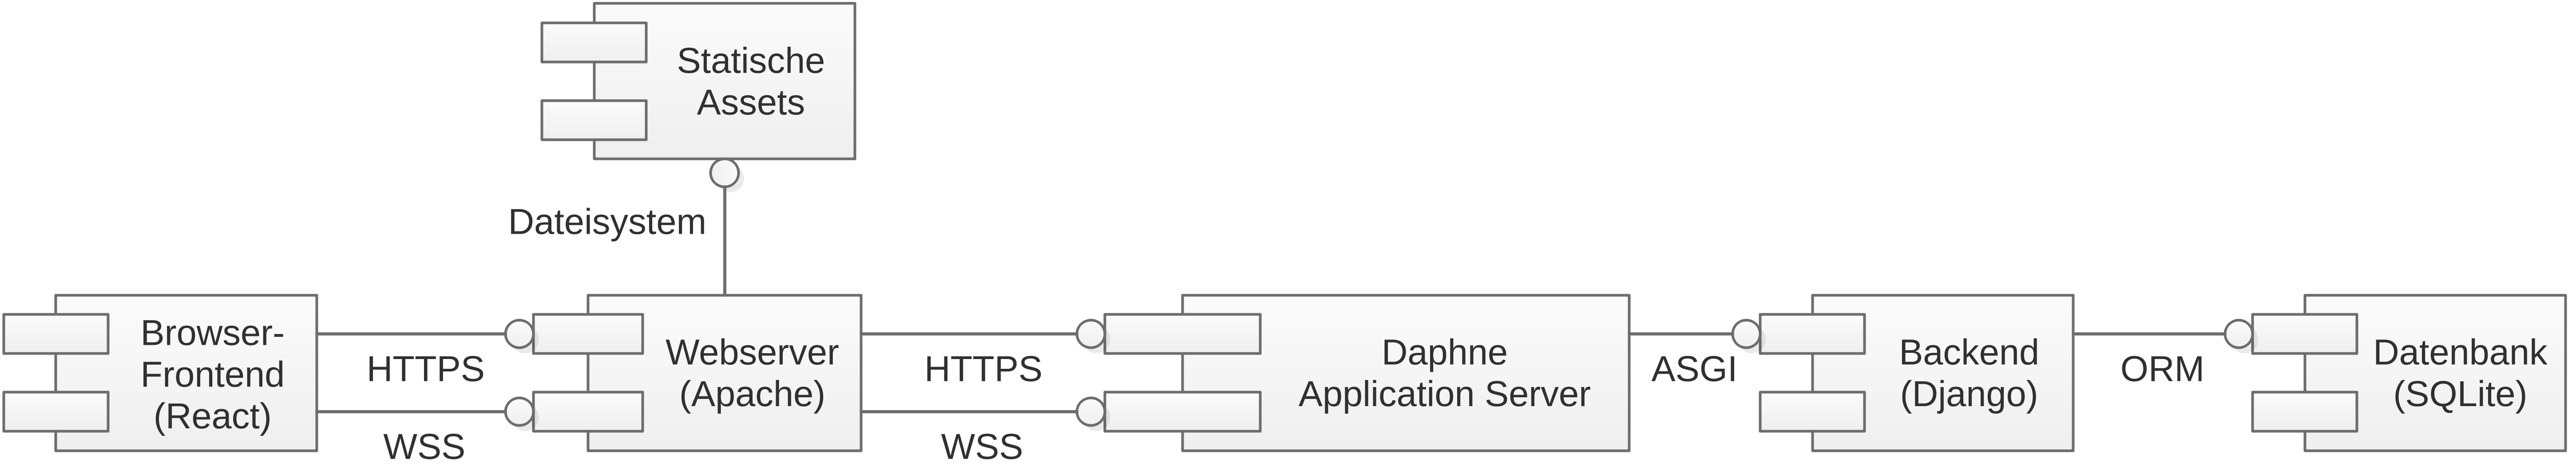
\includegraphics[width=\textwidth]{deployment}
		\caption{Systemkomponenten und Schnittstellen}
		\label{fig:components}
	\end{figure}
	
	Abbildung \ref{fig:components} zeigt die Systemkomponenten, die im folgenden beschrieben werden.
	
	\begin{itemize}
		\item Die \textit{SQLite}-Datenbank stellt die Datenhaltung dar. Sie speichert die fachlichen Entitäten und Beziehungen in Tabellen.
		\item Das mit dem \textit{Django-Framework} entwickelte Backend implementiert die Spiellogik und steuert den Benutzerzugriff. Es greift über den Object Relational Mapper (ORM) auf die Datenbank zu.
		\item Der \textit{Daphne Application Server} stellt die Laufzeitumgebung für das Django-Backend bereit. Er kommuniziert mit dem Backend über das Asynchronous Server Gateway Interface (ASGI), einem Standard zur Server-Anbindung asynchroner Python-Web-Apps.
		\item Der vom Hoster Uberspace bereitgestellte Apache-Webserver bindet als Reverse Proxy das Backend an das öffentliche Internet an. Er kommuniziert über HTTPS bzw. verschlüsselte WebSockets (WSS) mit dem Application Server und stellt statische Assets (HTML, CSS, JS, Grafiken) direkt aus dem Dateisystem zur Verfügung.
		\item Das React-Frontend wird über HTTPS vom Server geladen und im Browser ausgeführt. Es kommuniziert per GraphQL mit dem Backend und nutzt dabei sowohl das HTTPS-, als auch das WSS-Protokoll.
	\end{itemize}
	
	
	\section{Daten}
	
	\begin{figure}
		\centering
		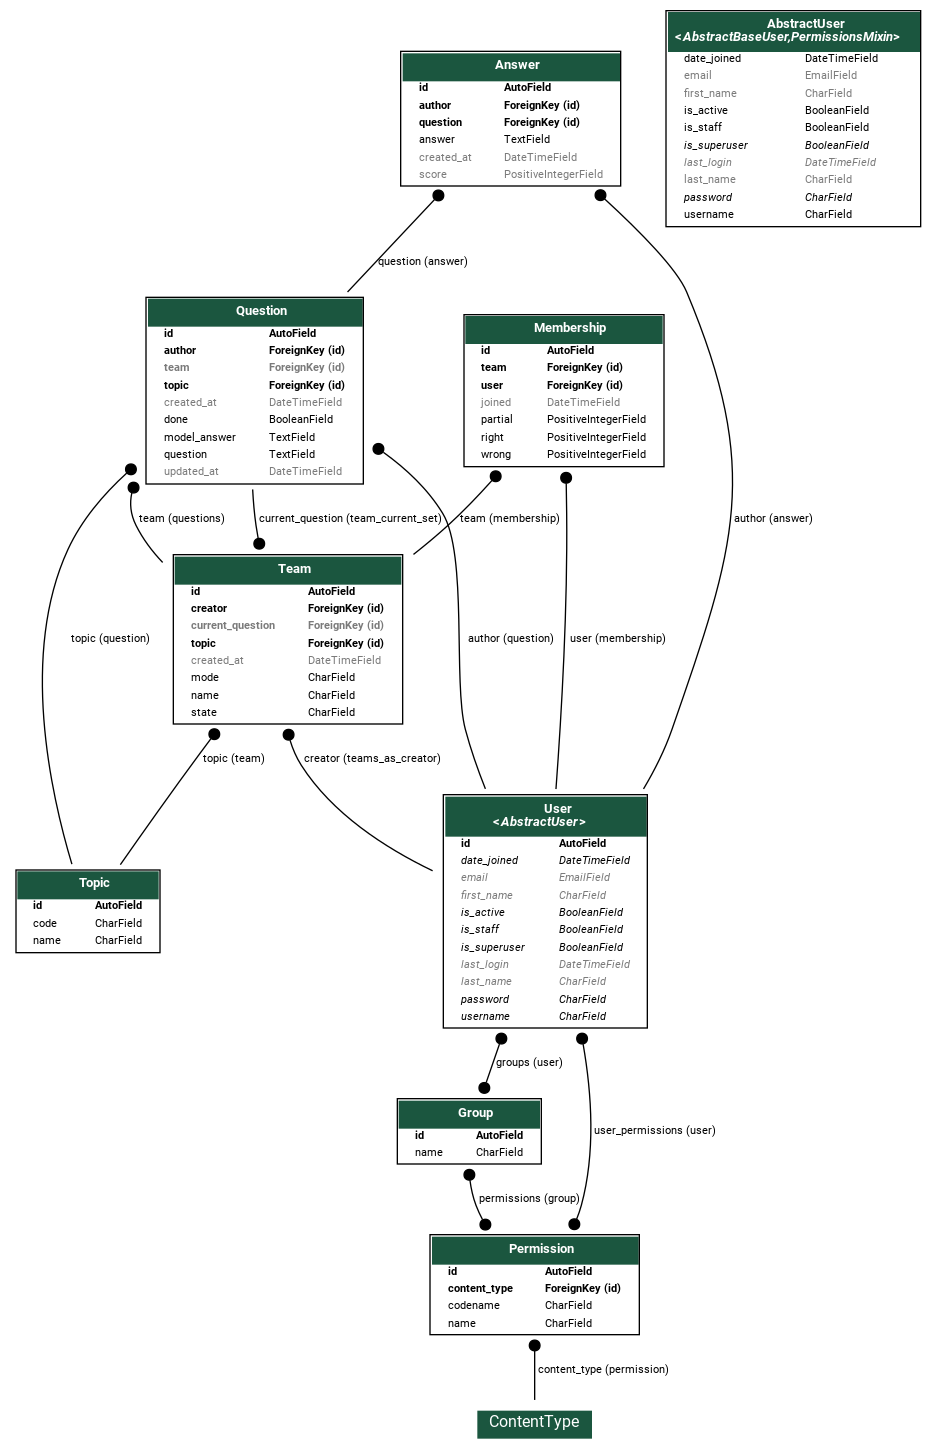
\includegraphics[width=\textwidth]{models_final}
		\caption{Finale Datenbankstruktur}
		\label{fig:database}
	\end{figure}

	Abbildung \ref{fig:database} zeigt die finale Datenbankstruktur der Applikation.
	
	Die bereits im Bericht zu Meilenstein 3 vorgestellte Grundstruktur ist deutlich zu erkennen, allerdings wurde das Modell im Verlauf des erkenntnisgetriebenen Entwicklungsprozesses weiter verfeinert und angepasst.
	
		\subsection{Team}
	Die Klasse \textit{Team} ist das Herzstück der Quiz-App. Sie bildet ein Team von Benutzern ab, die zusammen spielen. Außerdem speichert sie den Benutzer, der das Team erstellt hat (\textit{creator}), enthält einen frei wählbaren Namen (\textit{name}) und wird einem Thema (\textit{topic}) zugeordnet.
	
	Das Feld für den Spielmodus (\textit{mode}) kann die Werte \texttt{train} (Trainingsmodus) oder \texttt{competition} (Wettkampf) annehmen.
	
	Ein Team befindet sich immer in einem definierten Zustand (\textit{state}):
	
	\begin{itemize}
		\item \texttt{open}: Das Team wurde erstellt und kann Mitglieder aufnehmen.
		\item \texttt{question}: Diese Phase stellt die \textit{Erarbeitungsphase} dar. In dieser Phase erarbeiten die Teammitglieder fachliche Fragen für ihre Mitspieler. 
		\item \texttt{answer}: In dieser Phase müssen die Spieler die erarbeiteten Fragen beantworten. Das System wählt die jeweils zu bearbeitende Frage zufällig aus und hinterlegt sie im Feld \textit{current\_{}question}.
		\item \texttt{scoring}: Bei Eintritt in die \textit{Bewertungsphase} haben die Spieler ihre Antworten eingegeben und es erfolgt die Bewertung durch den Fragesteller. Sind noch unbeantwortete Fragen in der Runde vorhanden, so wechselt die Runde wieder in den Zustand \texttt{answer}.
		
		\item \texttt{done}: Diese Phase markiert den Abschluss der Runde. Spielern wird abhängig vom gewählten Spielmodus nur eine persönliche oder eine gesamte Statistik der Leistung des Teams angezeigt. In dieser Phase können Mitglieder hinzugefügt oder entfernt werden und der Modus gewechselt werden. Das Team wechselt ausgehend von dieser Phase wieder in die Phase \textit{question}, falls eine neue Runde gespielt werden soll.
		
	\end{itemize}
	
	\subsection{Membership}
	Die Klasse \textit{Membership} bildet die Mitgliedschaft eines Benutzers (\textit{user}) in einem Team (\textit{team}) ab.
	Die Attribute \textit{right}, \textit{wrong} und \textit{partial} speichern die Anzahl der Fragen, die der Nutzer in der aktuellen Runde richtig, falsch bzw. teilweise richtig beantwortet hat. 
	
	\subsection{Question}
	Die Klasse \textit{Question} bildet eine fachliche Frage ab. Sie speichert den Autor (\textit{author}) der Frage, den Fragetext (\textit{question}), das zugehörige Thema (\textit{topic}), die Musterantwort (\textit{model\_{}answer}) und eine Referenz auf das Team.
	
	\subsection{Answer}
	Die Klasse \textit{Answer} enthält die Antwort (\textit{answer}) eines Spielers (\textit{author}) auf eine Frage (\textit{question}). Sie speichert außerdem die durch den Fragesteller vergebene Bewertung (\textit{score}).
	
	\subsection{Topic}
	Die Klasse \textit{Topic} stellt ein fachliches Thema dar. Hier wurde beispielhaft eine Liste der an der IUBH verfügbaren Module hinterlegt. Das Attribut \textit{name} speichert die Kursbezeichnung, das Attribut \textit{code} den Modulcode. Diese Klasse dient der besseren Strukturierung der Fragen in der \textit{Knowledge Base}.

	\subsection{User}
	Die Klasse \textit{User} entspricht dem unveränderten Benutzermodell des Django-Frameworks. Details dazu finden sich in der Django-Dokumentation\footnote{https://docs.djangoproject.com/en/3.0/ref/contrib/auth/}.	
	
	\section{GUI}
	
	\begin{figure}
		\centering
		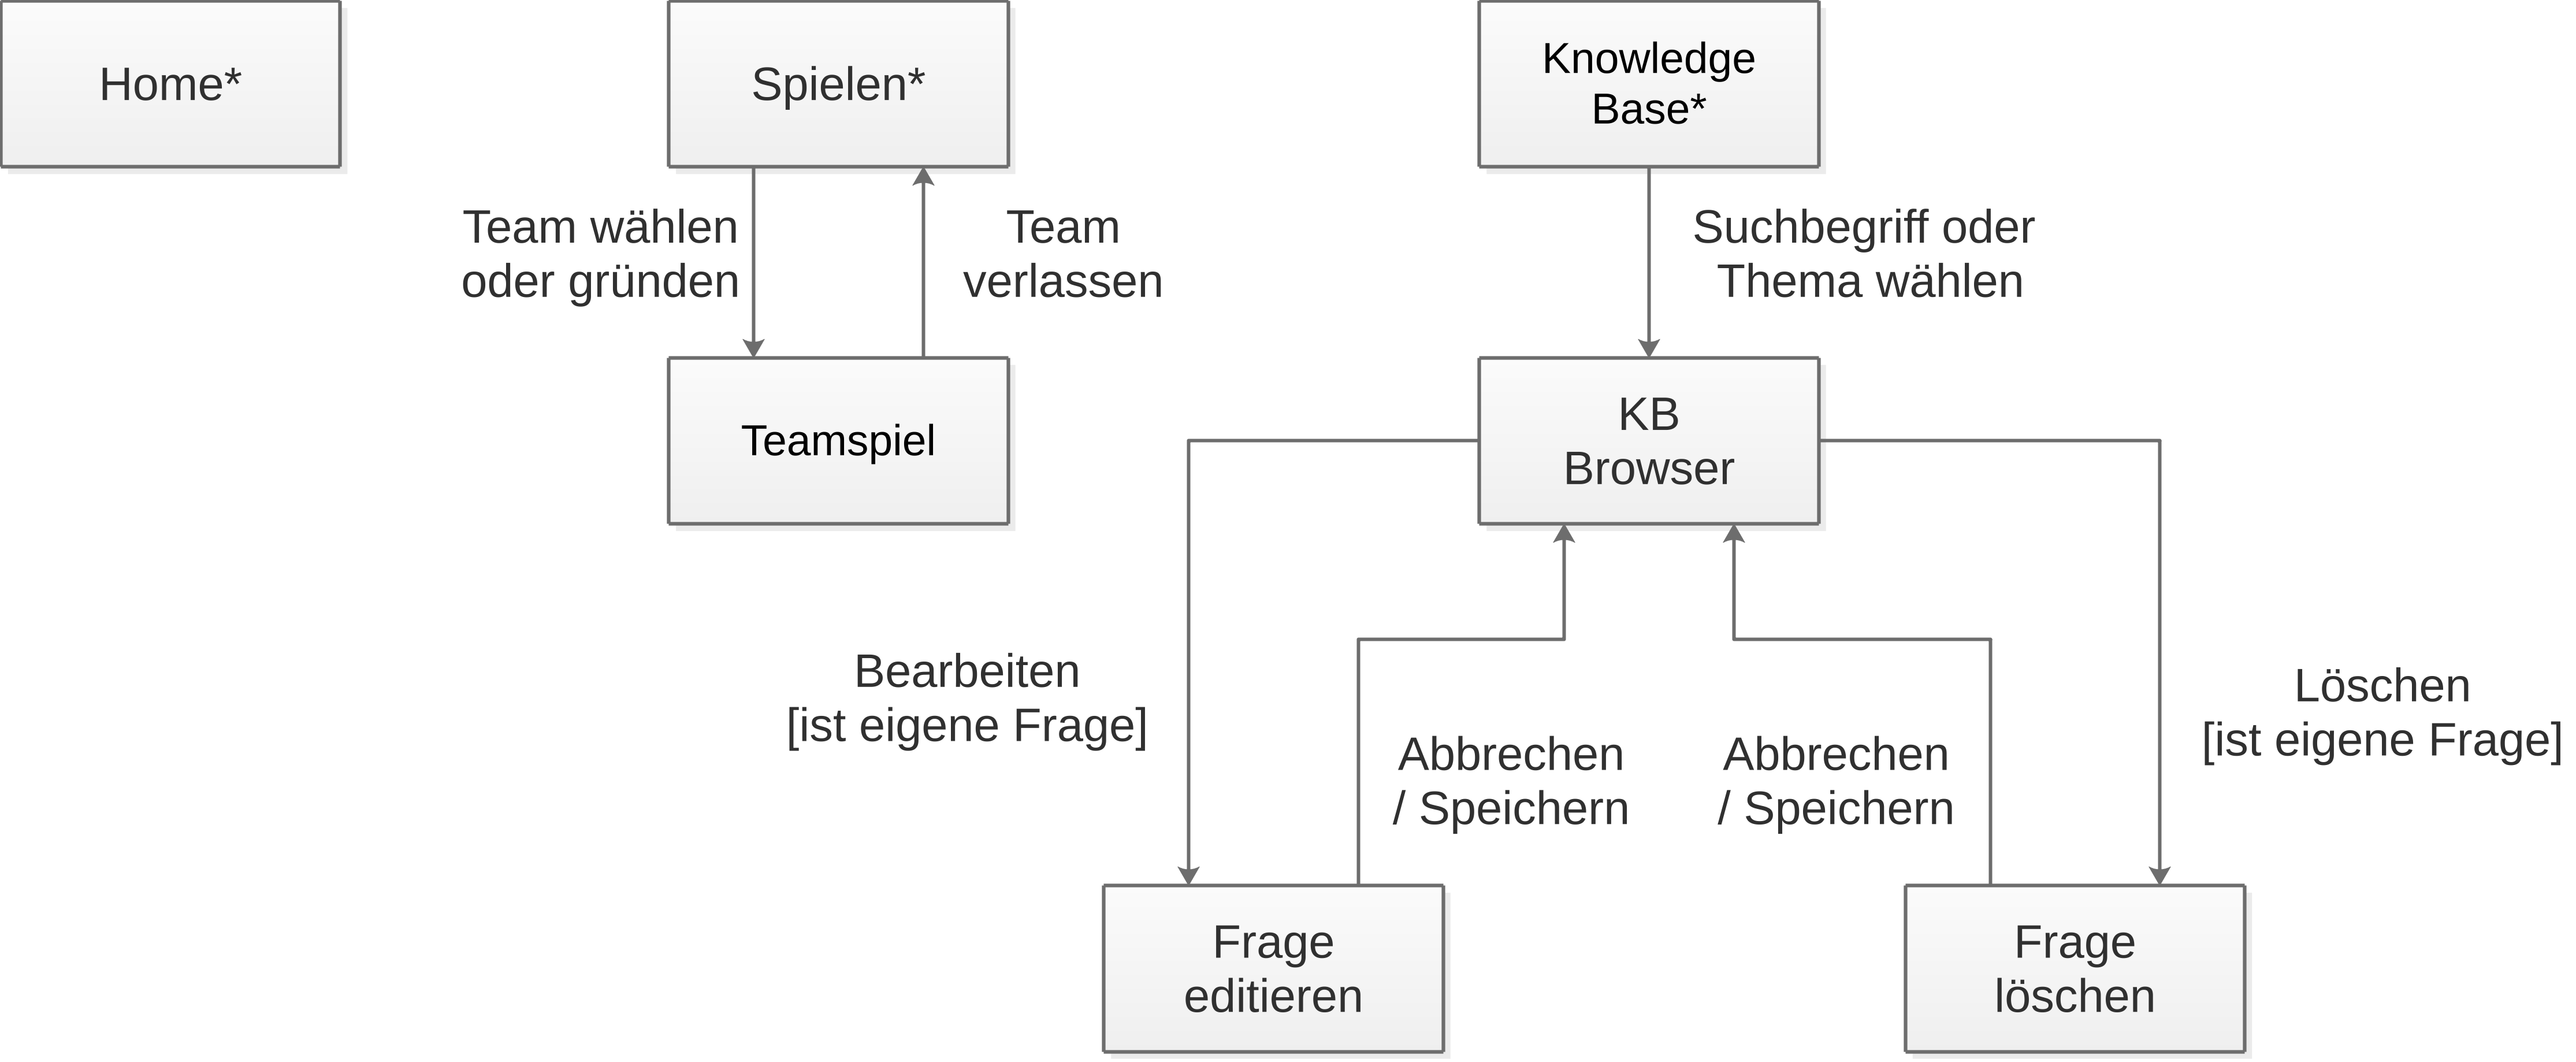
\includegraphics[width=\textwidth]{gui.png}
		\caption{GUI-Masken und Übergänge}
		\label{fig:gui}
	\end{figure}
	
	Dieser Abschnitt beschreibt in Kürze den Aufbau und das Zusammenspiel der GUI-Masken der App. Für weitere Details sei auf das Benutzerhandbuch verwiesen.
	
	Das Zusammenspiel der GUI-Masken in der App ist in Abbildung \ref{fig:gui} schemenhaft dargestellt. Die mit Sternchen (*) markierten Masken sind über die Navigation der App direkt erreichbar und somit kann ein Wechsel zur entsprechenden GUI-Maske über einen Klick auf den Link von jeder beliebigen Stelle der App ausgelöst werden -- diese Übergänge wurden aus Gründen der Übersichtlichkeit in der Grafik nicht eingezeichnet.
	
	Auch die Masken für Login und Logout werden an dieser Stelle ausgelassen.
	
	Die grafische Oberfläche gliedert sich in drei Hauptbereiche:
		
	\subsection{Home}
	Der Bereich \textit{Home} ist die Landing Page des Q-Teams-Projektes. Sie stellt mithilfe des Projektvideos das Konzept vor.

	\subsection{Spielen}
	Im Bereich \textit{Spielen} findet sich eine Übersicht über die Teams, in denen der Benutzer Mitglied ist. Darüber hinaus kann er an dieser Stelle eigene Teams erstellen.
	
	Hat er ein Team erstellt oder wählt eines aus, so gelangt er zur Maske \textit{Teamspiel}.
	
	\subsubsection{Teamspiel}	

	\begin{figure}
		\centering
		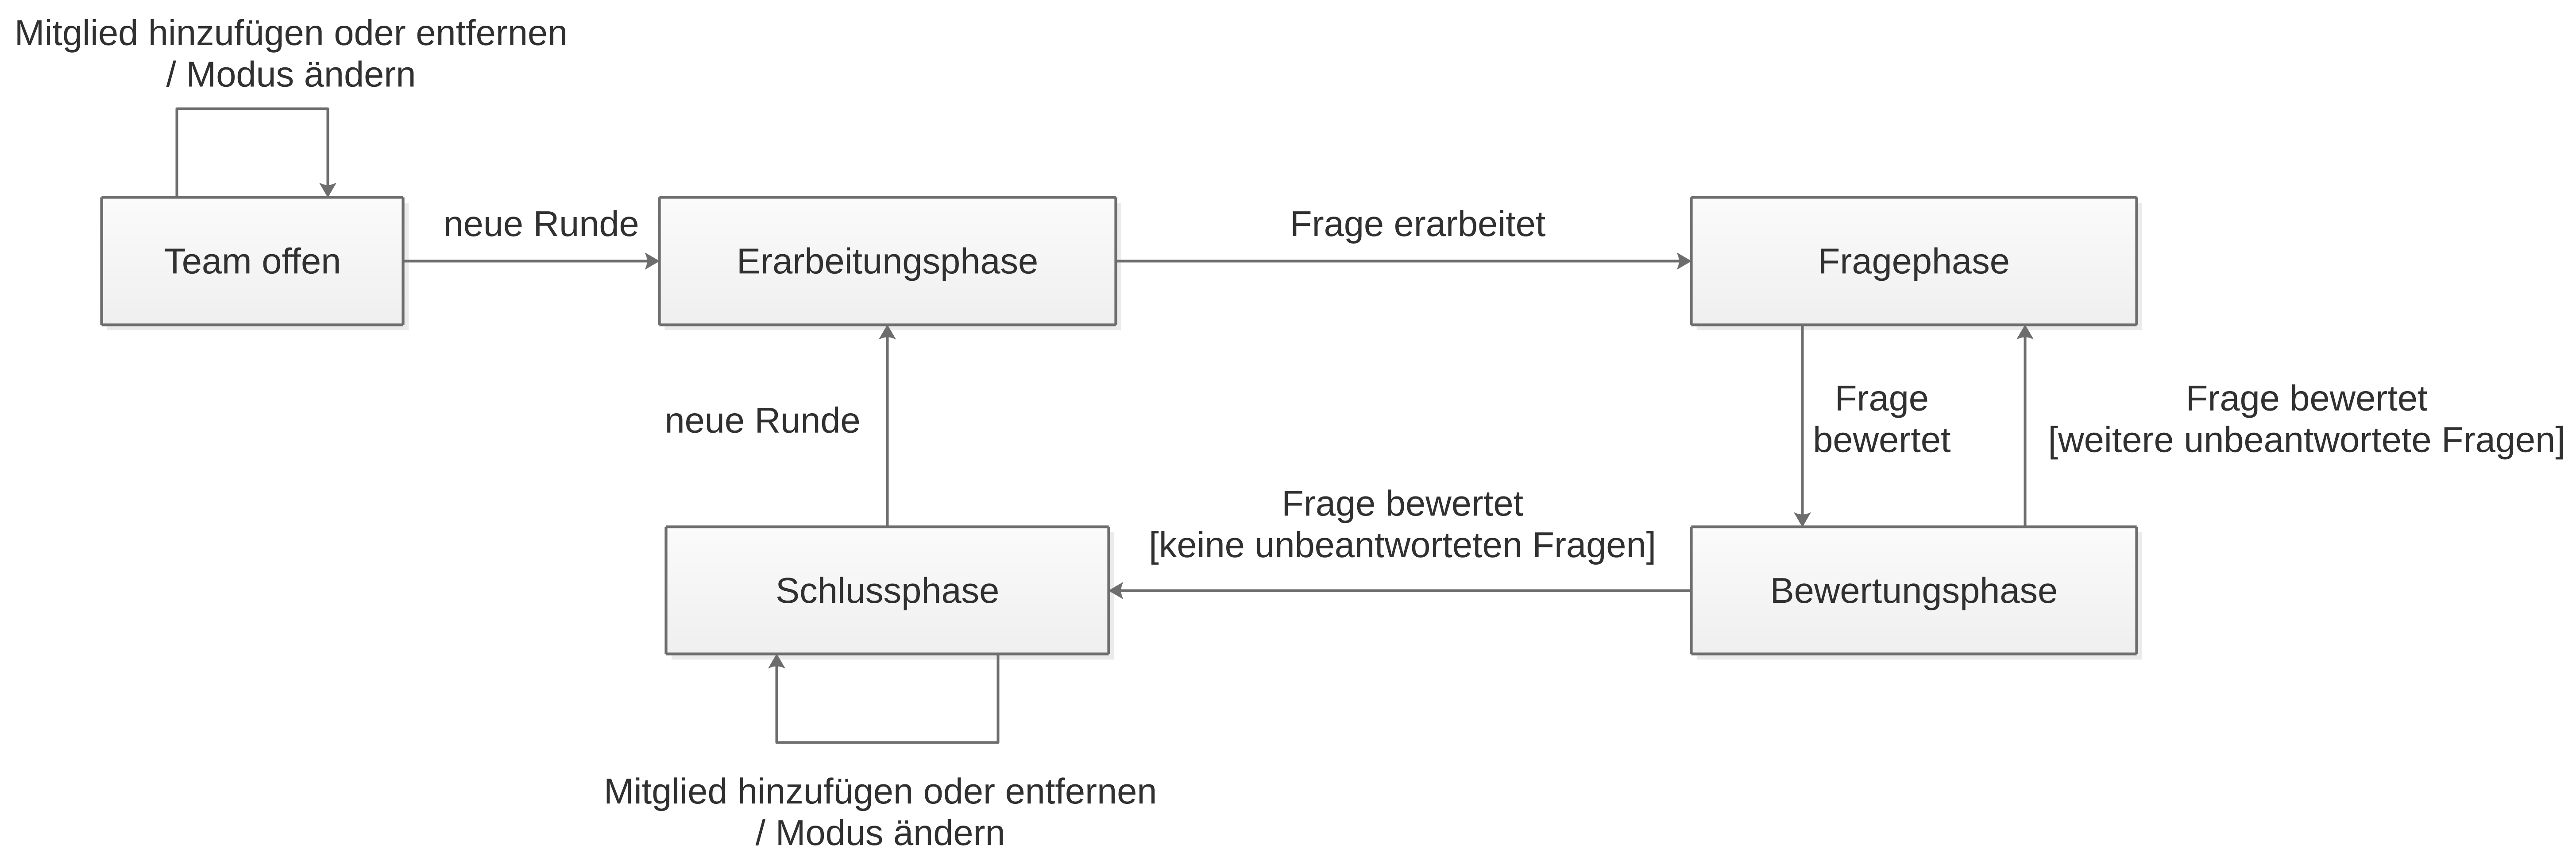
\includegraphics[width=\textwidth]{ablauf}
		\caption{Phasen des Spiels}
		\label{fig:phasen}
	\end{figure}
		
	Diese Seite ist der Kern der Applikation, denn dort findet das eigentliche Quiz statt. Abhängig von der jeweiligen Phase des Spiels sind an dieser Stelle verschiedene Funktionen verfügbar. Ablauf und Funktionen sind in Abbildung \ref{fig:phasen} skizziert.
	
	
	\subsection{Knowledge Base}
	Die \textit{Knowledge Base} stellt den Zugang zu bereits gespielten Fragen aller Spieler bereit und dient als Inspiration für eigene fachliche Fragen.
	
	Auf der Übersichtsseite der Knowledge Base kann der Nutzer einen Suchbegriff eingeben oder ein Thema wählen. Sodann gelangt er auf die Seite \textit{Knowledge Base Browser}.
	
	\subsubsection{Knowledge Base Browser}
	Diese Seite gibt das Suchergebnis mit den gefundenen Fragen und Musterantworten aus und bietet weitere Filtermöglichkeiten.
	
	Ist der aktuelle Nutzer auch der Autor einer Frage, so hat er die Möglichkeit, diese zu editieren oder zu löschen. Nach einem Klick auf den entsprechenden Button gelangt er dazu auf die Seite \textit{Frage editieren} bzw. \textit{Frage löschen}.

	\setcounter{chapter}{0}
	
	
	
	% ANHANG
	\begin{appendices}
	\renewcommand{\appendixtocname}{Anhang}
	\renewcommand{\appendixpagename}{Anhang}
	\appendixpage	
	\addappheadtotoc
	\chapter{Anforderungen}	
		
		\section{Funktionale Anforderungen}
		
	\subsection{Als Spieler möchte ich mit dem Quizsystem gezielt fachliche Inhalte wiederholen, um mich auf
Prüfungen vorzubereiten.}

		\begin{tabularx}{\textwidth}{Xr}
			
			Kriterien & Erfüllungsgrad \\
			\midrule
		Das Thema einer Quizrunde kann vor Beginn festgelegt werden. &  Voll umgesetzt\\
		Die Module der IUBH können als Thema ausgewählt werden. & Voll umgesetzt \\
		Die Lernzyklen der Module können als Thema ausgewählt werden. & Nicht umgesetzt \\
			\bottomrule
		\end{tabularx}		
		
		\subsection{Als Spieler möchte ich gegen einen anderen Spieler antreten können, um mich mit ihm zu messen /
vergleichen.}

		\begin{tabularx}{\textwidth}{Xr}
			
			Kriterien & Erfüllungsgrad \\
			\midrule
		Das Spiel kann mit anderen Menschen gespielt werden. & Voll umgesetzt \\
		Es kann ein kompetitiver Spielmodus festgelegt werden. & Voll umgesetzt \\
		Den Spielern werden ceteris paribus dieselben Fragen gestellt. & Voll umgesetzt \\		
		Die Antworten werden mit Punkten bewertet. & Voll umgesetzt \\
		Den Spielern wird eine Übersicht mit ihren Punkte angezeigt. & Voll umgesetzt \\
			\bottomrule
		\end{tabularx}	
		
		\subsection{Als Spieler möchte ich mit einem anderen Spieler gemeinsam spielen, um mich im Team über Lerninhalte austauschen zu können.}	
			\begin{tabularx}{\textwidth}{Xr}
			
			Kriterien & Erfüllungsgrad \\
			\midrule
		Das Spiel kann mit anderen Menschen gespielt werden. & Voll umgesetzt \\
		Es kann ein Team gebildet werden. & Voll umgesetzt \\
		Es kann ein kooperativer Spielmodus festgelegt werden. & Voll umgesetzt \\
			\bottomrule
		\end{tabularx}	
		
		\subsection{Als Spieler möchte ich Fragen und Antworten für andere Spieler hinzufügen und pflegen, um mein
Wissen weiterzugeben und zu festigen.}
		\begin{tabularx}{\textwidth}{Xr}
			
			Kriterien & Erfüllungsgrad \\
			\midrule
		Fragen und Antworten können persistiert werden. & Voll umgesetzt \\
		Persistierte Fragen und Antworten können angepasst werden. & Voll umgesetzt \\
		Persistierte Fragen und Antworten können gelöscht werden. & Voll umgesetzt \\
		Persistierte Fragen und Antworten können angesehen werden. & Voll umgesetzt \\
		Persistierte Fragen und Antworten können in einer Spielrunde genutzt werden. & Voll umgesetzt\\
			\bottomrule
		\end{tabularx}		
		
		\subsection{Als Spieler möchte ich Feedback zu meiner Lösung bekommen, um aus Fehlern zu lernen.}
		\begin{tabularx}{\textwidth}{Xr}
			
			Kriterien & Erfüllungsgrad \\
			\midrule
			Die Antworten werden bewertet. & Voll umgesetzt \\
			Dem Spieler wird die Bewertung der Antwort angezeigt. & Voll umgesetzt \\
			
			\bottomrule
		\end{tabularx}	
		
		\section{Nicht-funktionale Anforderungen}
		
		\subsection{Als Spieler möchte ich das Quiz im Browser spielen können, damit ich es auf verschiedenen
Plattformen spielen kann und keine Zusatzsoftware installieren muss.}
		\begin{tabularx}{\textwidth}{Xr}
			
			Kriterien & Erfüllungsgrad \\
			\midrule
		\textit{Spielen} bedeutet hier den Ablauf einer Spielrunde in den Modi \textit{kompetitiv} und \textit{kooperativ} in einem Team mit 5 Spielern ohne Spielabbrüche durchzuspielen. 	
		Das Spiel ist mit folgenden Browsern in der Standardinstallation spielbar: & \\
		Quizrunde mit folgenden Browsern spielen: & \\
		IE 11.778.18362.0 & \\
		Firefox 76.0 & \\
		Edge 81.0.416.68 & \\
		Chrome 81.0.4044.138 & \\
			\bottomrule
		\end{tabularx}	
			
		\subsection{Als Auftraggeber wünsche ich mir einen lauffähigen Prototyp, damit ich die mögliche Einsatzfähigkeit in der Praxis evaluieren kann.}
		\begin{tabularx}{\textwidth}{Xr}
			
			Kriterien & Erfüllungsgrad \\
			\midrule
			Es kann im Browser Firefox 76.0 in einem Team mit 3 Spielern jeweils eine Spielrunde in den Modi \textit{kompetitiv} und \textit{kooperativ} durchgespielt werden. & \\
			Es kann im Browser Firefox 76.0 in der Erarbeitungsphase eine Frage mit Antwort persistiert werden. & \\
			Es können im Browser Firefox 76.0 in der Erarbeitungsphase die bereits persistierten Fragen mit Antworten angezeigt werden. & \\
			
			\bottomrule
		\end{tabularx}	
				
		\subsection{Als Auftraggeber / Spieler wünsche ich mir ein Benutzerhandbuch, um mir einen Überblick über
Aufbau und Funktionen des Systems verschaffen zu können.}
		\begin{tabularx}{\textwidth}{Xr}
			
			Kriterien & Erfüllungsgrad \\
			\midrule
		Das Benutzerhandbuch wird dem Auftraggeber zugestellt. & Voll umgesetzt\\
		Jede GUI-Maske wird mit einem Screenshot dargestellt und erläutert. & Voll umgesetzt\\
		Die Spielregeln werden erklärt. & Voll umgesetzt\\
			\bottomrule
		\end{tabularx}	
		
		\subsection{Als Auftraggeber / Betreiber wünsche ich mir eine Dokumentation zur Installation und
Inbetriebnahme, damit ich das Quiz ohne großen Aufwand den Studierenden zur Verfügung stellen
kann.}
		\begin{tabularx}{\textwidth}{Xr}
			
			Kriterien & Erfüllungsgrad \\
			\midrule
		Die Dokumentation wird dem Auftraggeber zugestellt. & Voll umgesetzt \\
		Die Dokumentation steht einem potenziellen Betreiber zur Verfügung. & Voll umgesetzt \\
		Die Dokumentation beschreibt die notwendige Hardware zur Installation und Inbetriebnahme. & Voll umgesetzt \\
		Die Dokumentation beschreibt die notwendige Software zur Installation und Inbetriebnahme. & Voll umgesetzt \\
		Die Dokumentation beschreibt die notwendigen Schritte zur Installation und Inbetriebnahme. & Voll umgesetzt \\
		
			\bottomrule
		\end{tabularx}	

		
			
		
		
		
	
	\chapter{Qualitätsziele}
	\label{chap:qziele}
	
	Im Bericht zu Meilenstein 3 wurden bereits Qualitätsziele festgelegt. Diese werden an dieser Stelle wieder aufgegriffen und deren Umsetzung beschrieben.
	
	\section{Funktionalität}
	
	\subsection{Die Quiz-App soll den fachlichen Prozess korrekt abbilden.}
	Der fachliche Prozess konnte wie geplant in der Applikation abgebildet werden.	
	
	\subsection{Das System soll gegenüber Bedrohungen von innen und außen gesichert sein.} 
	Der Zugriff auf das System ist ausschließlich verschlüsselt per HTTPS / WSS und SSH möglich. Benutzerkennwörter müssen die in Meilenstein 3 definierten Kennwortrichtlinien erfüllen. Die Speicherung der Kennwörter in der Datenbank erfolgt in verschlüsselter Form. Alle Datenbankzugriffe werden über den Object Relational Mapper (ORM) gekapselt. Benutzer erhalten nur die Zugriffsrechte, die zum Spielen des Quiz zwingend benötigt werden.
	
	\section{Benutzbarkeit}
	\subsection{Die Bedienung des Systems soll leicht erlernbar und möglichst intuitiv verständlich sein.}
	Die Bedienung des Systems ist so gestaltet, dass sie weitestgehend selbsterklärend ist. Das Projektvideo wurde auf der Startseite integriert, so dass Nutzer sich vor dem Spielbeginn mit dem Spielprinzip vertraut machen können. Auch ein Benutzerhandbuch steht bereit.
	\subsection{Die Oberfläche soll simpel und ansprechend gestaltet sein}
		Die Gestaltung der Oberfläche wurde an das Corporate Design der IUBH angelehnt, so dass für Studierende ein Wiedererkennungswert und eine Vertrautheit geschaffen wird. Die Dialogflüsse wurden klar und einfach strukturiert. Systemfunktionen sind immer über einen eindeutigen Weg zugänglich -- Redundanzen wurden vermieden.
		
	
	\section{Änderbarkeit}
	
	\subsection{Der Prototyp soll einfach erweiterbar sein und zu einem späteren Zeitpunkt zu einem ausgereiften Produkt ausgebaut werden können.}
	Mit React und Django wurden weit verbreitete Standard-Technologien eingesetzt, die mit ihrem modularen und komponentenbasierten Ansatz eine einfache Weiterentwicklung -- auch durch neu hinzukommende Entwickler -- gewährleisten. Der Quellcode ist kommentiert, die API-Dokumentation ist direkt über den interaktiven GraphQL-Endpoint\footnote{https://api.qteams.team} zugänglich, Datenmodell und Prozesse wurden in diesem Bericht dokumentiert.
	
		\subsection{Die Grundfunktionen des Systems sollen einfach getestet werden können.}
		Ein Quiz-Durchlauf kann mithilfe von zwei Browsern und zwei Demo-Benutzerkonten innerhalb weniger Minuten simuliert werden.
		
	
	\section{Effizienz}
		\subsection{Mit Serverressourcen soll schonend umgegangen werden.}
		Datenbankzugriffe wurden grundlegend optimiert: Es werden Indizes verwendet und wenn erforderlich datenbankseitige Aggregation. Ein ausführliches Profiling der Datenbankzugriffe findet allerdings im Kontext der prototypischen Umsetzung nicht weiter statt.		
		
		\subsection{Da es sich um eine interaktive Anwendung handelt, sollten Antwortzeiten des Systems niedrig gehalten werden.}
		Im exemplarischen manuellen Test lag die Antwortzeit der API in der Regel unter 100 ms. Ein nach subjektivem Ermessen verzögerungsfreies Arbeiten mit dem System ist möglich. 
	
	\section{Übertragbarkeit}

	\subsection{Das System soll einfach und unkompliziert bei einem Hosting-Provider installiert werden können.}
	Das System wurde beispielhaft beim Hosting Provider \textit{Uberspace} eingerichtet -- es lässt sich jedoch auch bei jedem beliebigen anderen Anbieter betreiben. Dies können Clouddienste wie z.B. Heroku, Netlify oder EC2 oder auch klassische Hoster wie Strato oder Hetzner sein.
	
	
	\subsection{Das System soll einfach in die Anwendungslandschaft einer Hochschule integrierbar sein.}
	Die modularen Komponenten zur Authentifizierung und Autorisierung sind einfach austausch- und erweiterbar, so dass eine Integration in die Anwendungslandschaft einer Hochschule über ein Single-Sign-On-System (z.B. via OAuth) problemlos möglich ist. 

	Auch Schnittstellen zum automatisierten Import von Modulbezeichnungen und -nummern (Themen) sind vorbereitet.	
	
	\section{Zuverlässigkeit}
	\subsection{Das System wird lediglich prototypisch umgesetzt, daher ist nur ein geringer Reifegrad gefordert.}
	Auf aufwändige automatisierte Tests wurde aufgrund der prototypischen Umsetzung und der begrenzten Ressourcen verzichtet. Mit ausführlichen, manuellen Tests auf verschiedenen Plattformen konnte aber sichergestellt werden, dass das System grundlegend funktioniert und ein einem Prototyp angemessener Reifegrad erreicht wurde.

	\subsection{Das System soll fehlerhafte Eingaben abfangen können.}
	GraphQL-API und ORM validieren alle Benutzereingaben und prüfen, ob die notwendigen Zugriffsrechte gegeben sind. Darüber hinaus werden Eingaben zusätzlich auch vom Frontend geprüft. Damit soll ein unvorhersehbares Verhalten des Systems durch schadhafte Eingaben vermieden werden.
	
	\chapter{Benutzerhandbuch}

	Wir freuen uns, dass du dich entschieden hast Q-Teams auszuprobieren. In diesem Benutzerhandbuch zeigen wir dir, wie Q-Teams aussieht und wie du es nutzen kannst! Dazu zeigen wir dir in einfachen Schritten, wie du deine erste Runde Q-Teams spielen kannst und wie du die Knowledge Base nutzt. Auf den Screenshots sind die wichtigsten Dinge farbig hervorgehoben: Eine purpurne Markierung zeigt eine Interaktionsmöglichkeit, hier musst du klicken oder tippen. Eine türkise Markierung weist dich auf wichtige Informationen hin.
	\newpage
	\section*{Schritt 1: Q-Teams starten}
	
	Um Q-Teams zu starten, rufe die Adresse \url{https://qteams.team} in deinem Browser auf. Am besten benutzt du einen aktuellen Firefox- oder Chrome-Browser auf deinem PC, aber auch mit anderen Browsern oder auf dem Smartphone kannst du Q-Teams nutzen.
	
	Nun sollte dich der Home-Bildschirm von Q-Teams begrüßen, siehe Abbildung \ref{fig:guide_home}. In unserem Projektvideo stellen wir dir Q-Teams vor. Du kannst das Video mit deinen Kommilitonen teilen, um sie zu überzeugen, mit dir in einem Q-Team zu lernen! In der Top-Leiste findest du jetzt nur den Home-Button und den Login-Button. Bist du eingeloggt, findest du hier zusätzlich die wichtigsten Funktionalitäten wieder: Spielen und Knowledge Base. Also, drücke auf den Login-Button, um dich einzuloggen!
	
	\begin{figure}[h!]
		\centering
		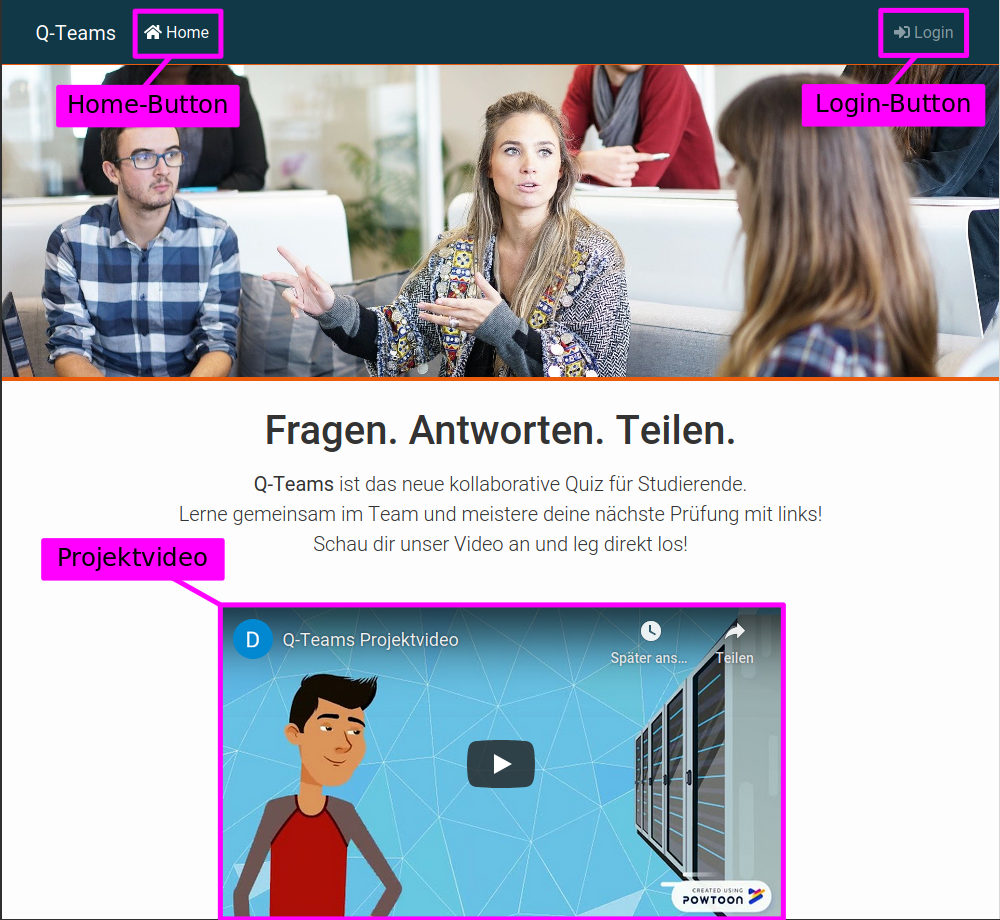
\includegraphics[width=\textwidth]{UserGuide/Home.png}
		\caption{Der Home-Bildschirm}
		\label{fig:guide_home}
	\end{figure}
	\newpage
	\section*{Schritt 2: Einloggen}
	
	Das Einloggen geht ganz einfach mit Benutzernamen und Passwort, die dir durch die IUBH zur Verfügung gestellt wurden. Die entsprechende Login-Maske in Abbildung \ref{fig:guide_login} ist dementsprechend einfach gehalten. Solltest du noch keine Login-Daten erhalten haben, wende dich an einen der Administratoren.
	
	\begin{figure}[h!]
		\centering
		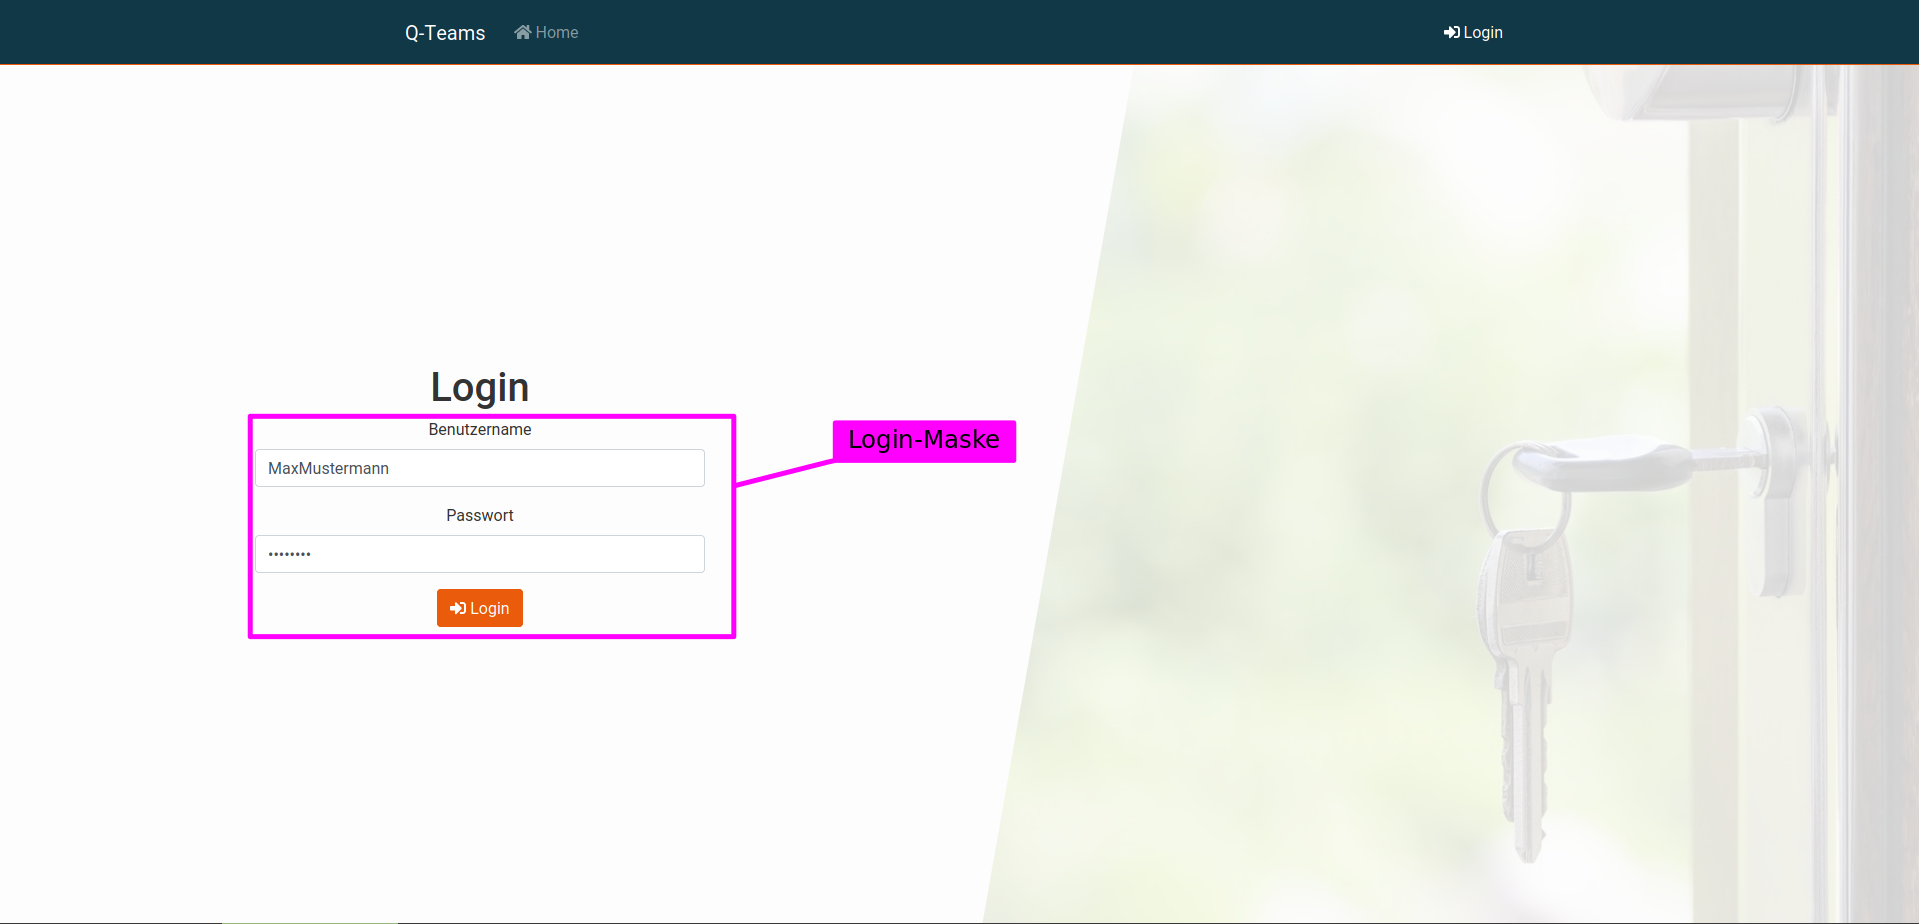
\includegraphics[width=\textwidth]{UserGuide/Login.png}
		\caption{Die Login-Maske}
		\label{fig:guide_login}
	\end{figure}
	
	\newpage
	\section*{Schritt 3: Q-Team gründen oder beitreten}
	
	Sobald du dich erfolgreich eingeloggt hast, siehst du den Spielen-Bildschirm aus Abbildung \ref{fig:guide_spielen}. Mit Hilfe der Eingabefelder in der unteren Hälfte kannst du nun ein neues Team gründen. Du musst lediglich den Teamnamen und das Thema des Teams festlegen. Als Thema wählst du eins der Module der IUBH. Alle Module der IUBH sind mit ihrer Kennung und ihrem Namen gespeichert (\zB IGIS01 Grundlagen der industriellen Softwaretechnik). So findest du mühelos dein passendes Thema. Hast du Namen und Thema gewählt, musst du nur auf den \textit{Team gründen} Button drücken\footnote{Der Name und das Thema des Teams lassen sich anschließend nicht mehr ändern.} und deine erste Runde Q-Teams startet automatisch. Bevor es damit weitergeht, zeigen wir dir, wie du mit einem bestehenden Team spielen kannst.
	
	In der oberen Hälfte des Spielen-Bildschirms werden dir alle Teams gezeigt, bei denen du Mitglied bist. Gezeigt werden der Teamname, das Thema des Teams und der Teamleiter\footnote{Der Spieler, der das Team gegründet hat.}. Durch Klicken auf den Teamnamen trittst du der aktuellen Runde in diesem Team bei.
	
	\begin{figure}[h!]
		\centering
		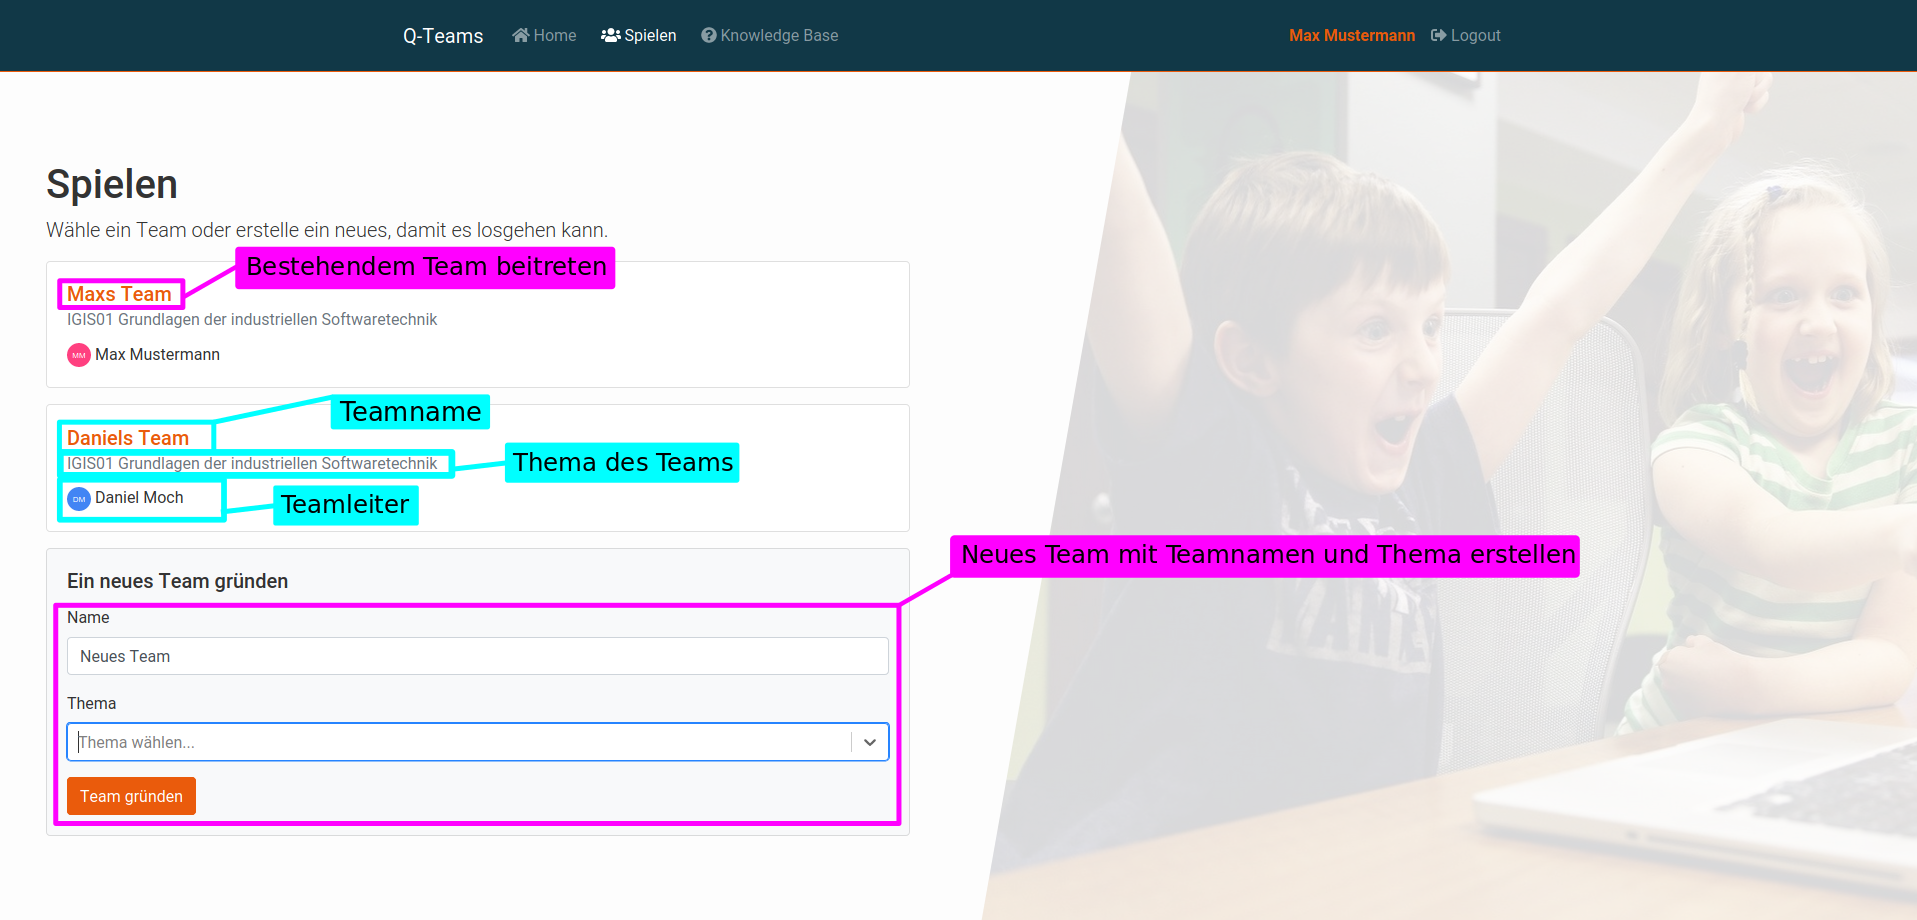
\includegraphics[width=\textwidth]{UserGuide/Spielen.png}
		\caption{Der Spielen-Bildschirm}
		\label{fig:guide_spielen}
	\end{figure}
	
	\newpage
	\section*{Schritt 4: Eine Runde Q-Teams beginnen}
	
	Ein neues Q-Team startet immer in der Phase \textit{Beginn des Spiels}. Als Teamleiter sieht das wie in Abbildung \ref{fig:guide_beginn_nichtbereit} aus. Auf der linken Seite werden alle Teammitglieder aufgelistet. Zu jedem Spieler werden der Vorname und Name, sowie der Benutzername gezeigt. Der Teamleiter ist besonders mit dem Schild-Icon gekennzeichnet. Zu deinem eigenen Namen und, je nach Spielmodus auch den anderen Spielern, werden die Anzahl der richtig/teilweise richtig/falsch beantworteten Fragen und der Punktestand angezeigt.
	
	Als Teamleiter kannst du, solange du alleine im Team bist, das Team verlassen und somit wieder löschen. Um spielen zu können müssen mindestens zwei Spieler im Team sein. Dazu fügst du Mitglieder durch Eingabe des Benutzernamens zum Team hinzu. Hier kannst du außerdem zwischen dem Trainings- und Wettkampfmodus umschalten.
	
	\begin{figure}[h!]
		\centering
		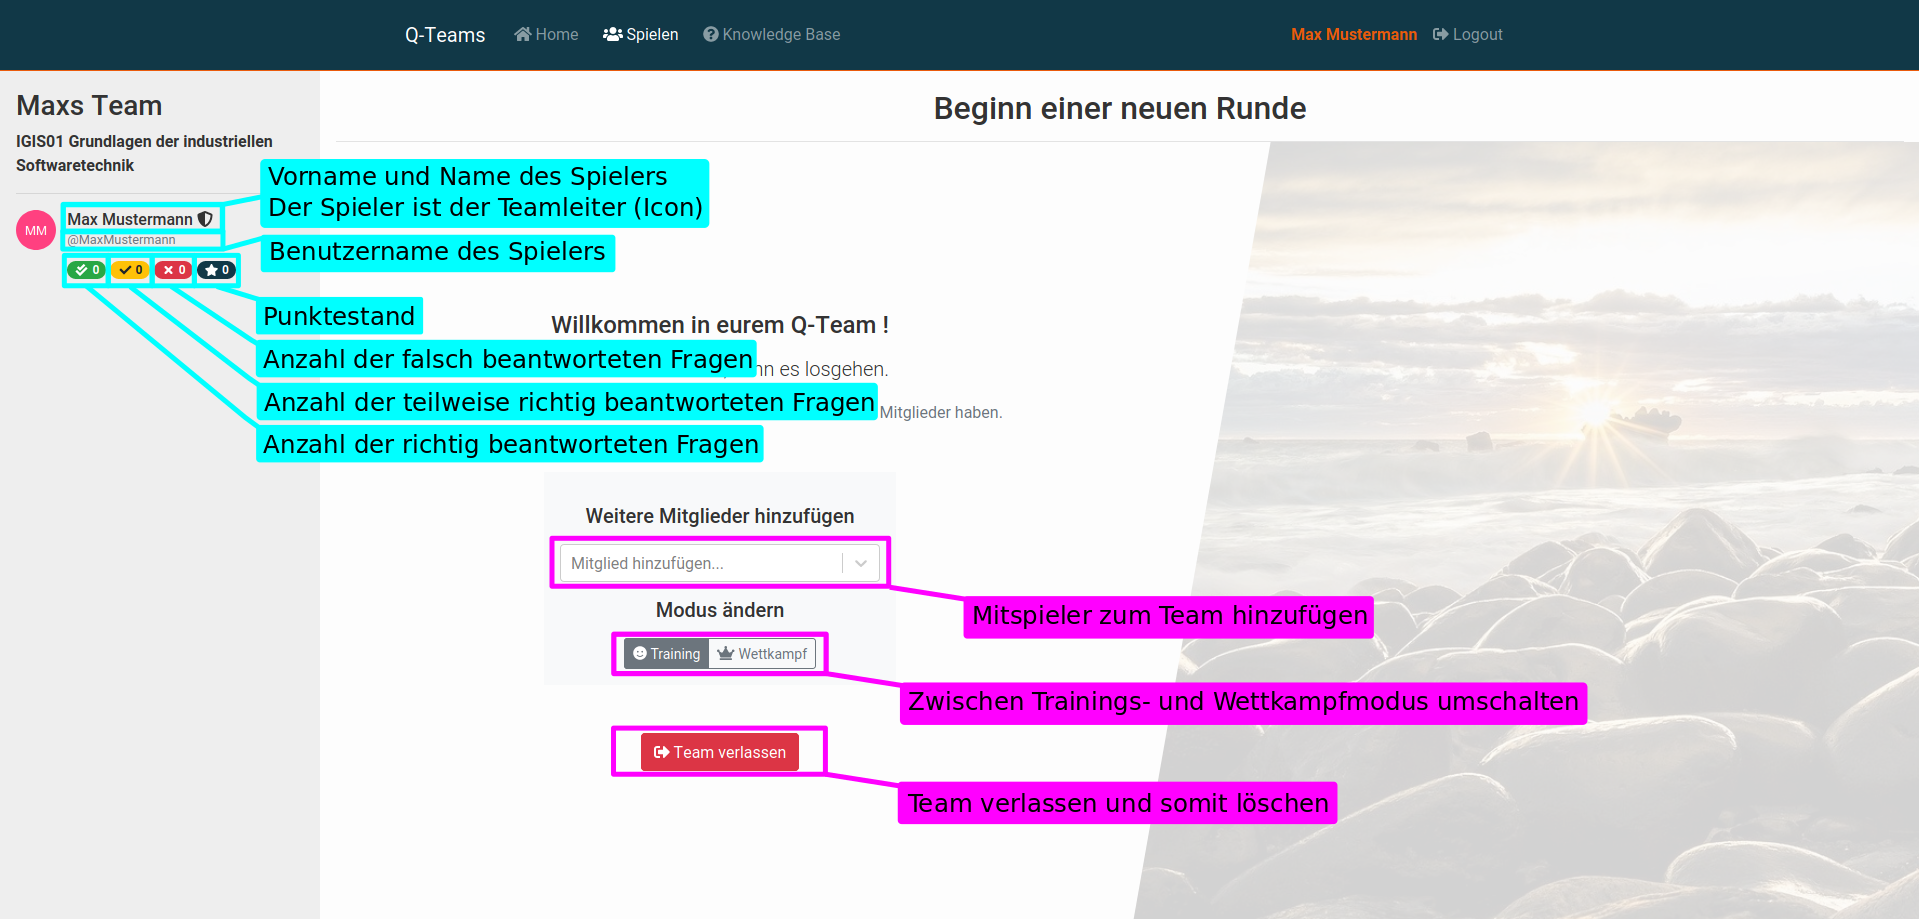
\includegraphics[width=\textwidth]{UserGuide/Rundenbeginn_Leiter.png}
		\caption{Die Phase Beginn des Spiels aus Sicht des Teamleiters mit nicht ausreichender Spielerzahl}
		\label{fig:guide_beginn_nichtbereit}
	\end{figure}
	
	Hast du einen weiteren Spieler zum Team hinzugefügt, kannst du die Runde durch Klicken auf den Button starten. In der Phase kannst du die anderen Spieler auch aus dem Team entfernen, dazu musst du auf den x-Button neben dem jeweiligen Namen klicken.
	
	\begin{figure}[h!]
		\centering
		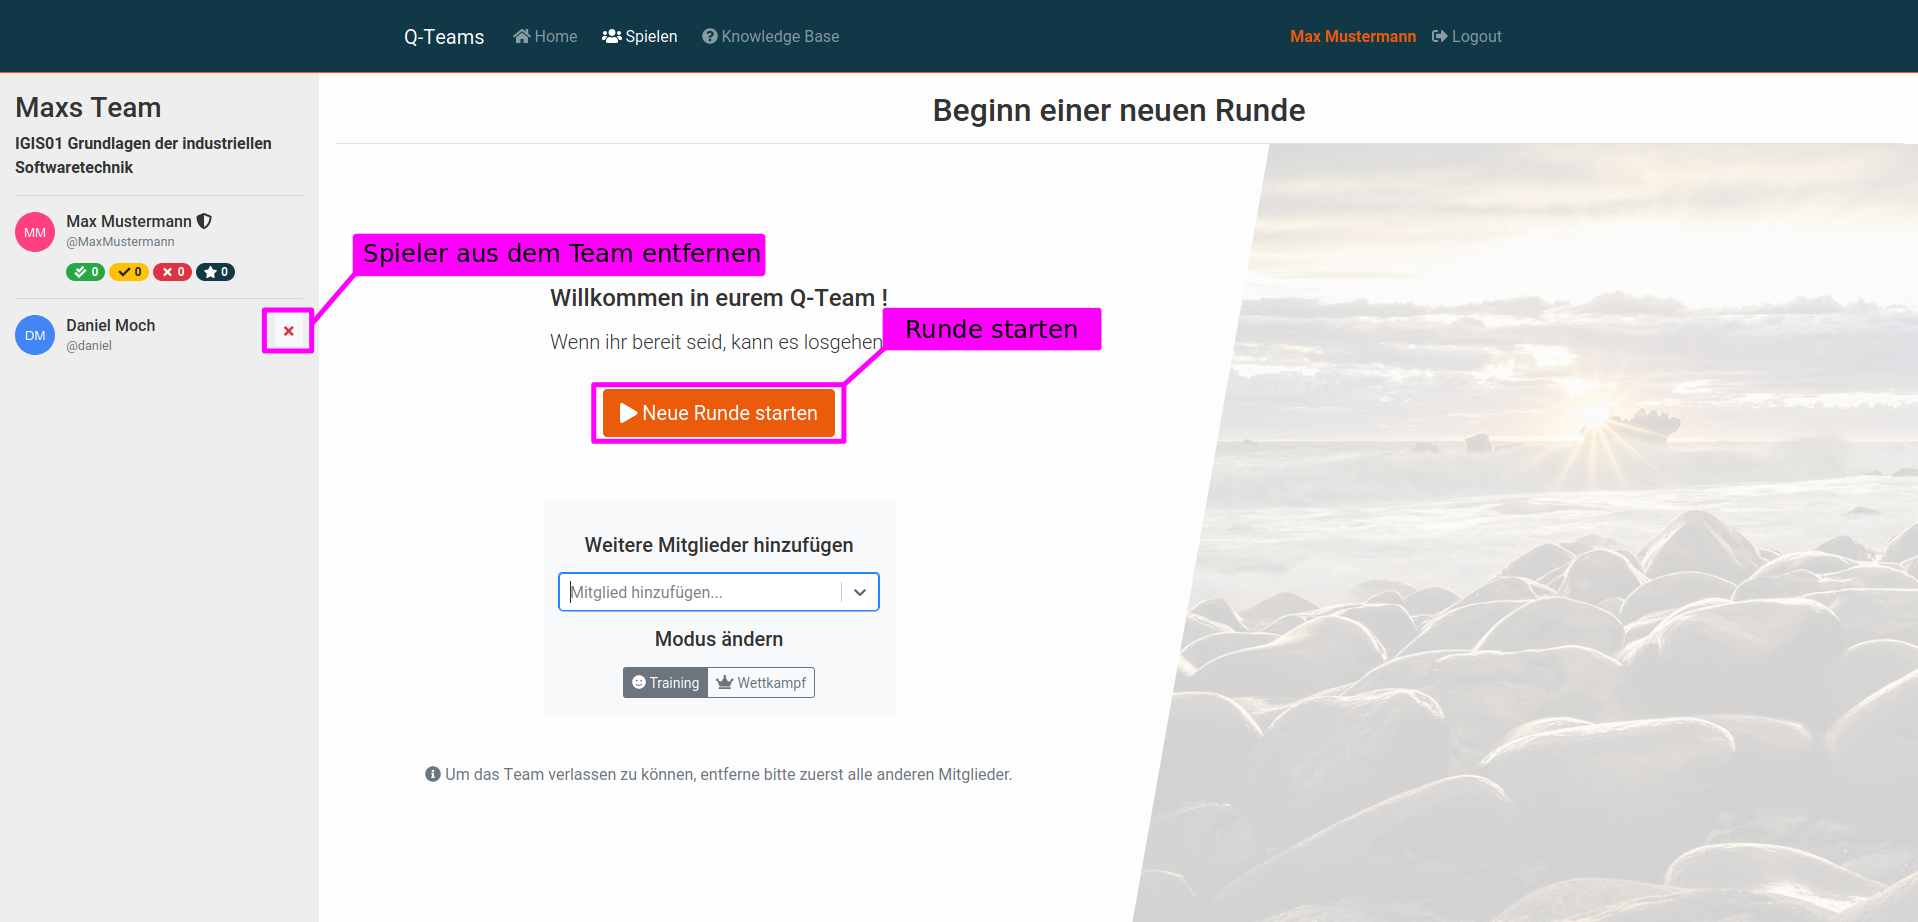
\includegraphics[width=\textwidth]{UserGuide/Rundenbeginn_Leiter_2.png}
		\caption{Die Phase Beginn des Spiels aus Sicht des Teamleiters mit ausreichender Spielerzahl}
		\label{fig:guide_beginn_bereit}
	\end{figure}
	
	Als Mitspieler in einem Team wird dir der Bildschirm aus Abbildung \ref{fig:guide_beginn_spieler} angezeigt. Wie du siehst, kannst du lediglich das Team verlassen oder darauf warten, dass der Teamleiter die Runde startet. Nur der Teamleiter sagt, wann es los geht!
	\begin{figure}[h!]
		\centering
		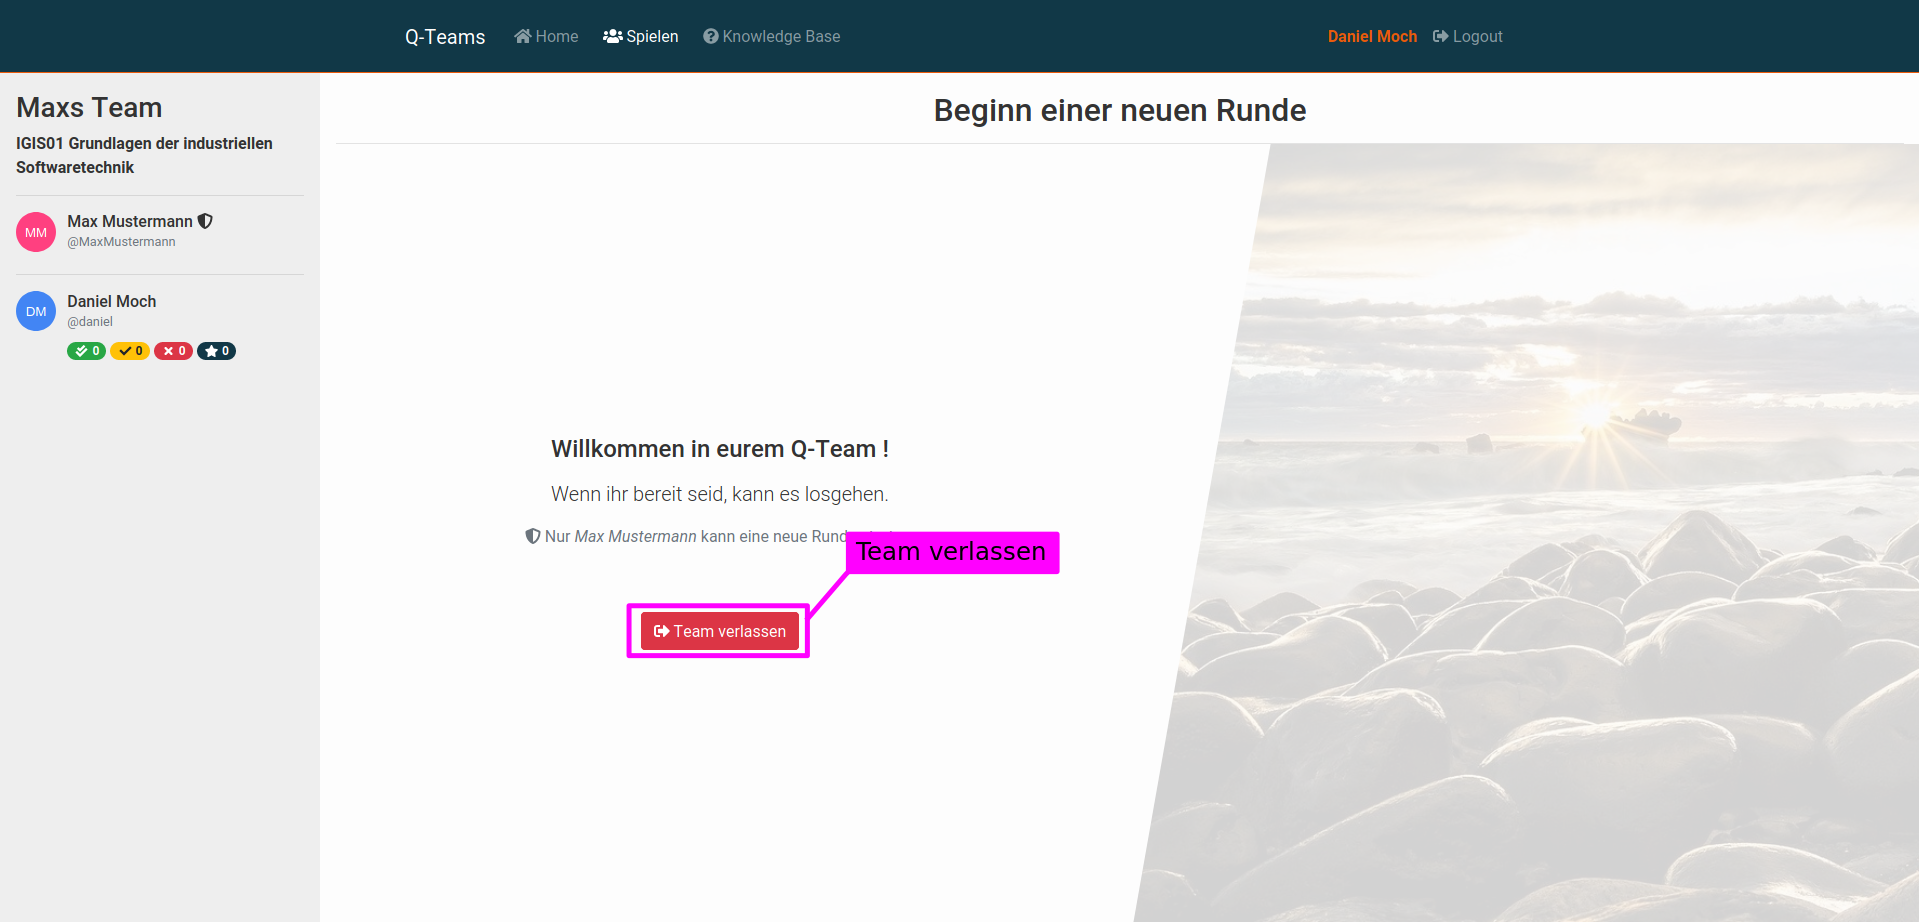
\includegraphics[width=\textwidth]{UserGuide/Rundenbeginn_Spieler.png}
		\caption{Die Phase \textit{Beginn des Spiels} aus Sicht eines Mitspielers}
		\label{fig:guide_beginn_spieler}
	\end{figure}
	
	\newpage
	\section*{Schritt 5: Die Frage erarbeiten}	
		
	Hast du oder der Teamleiter	 die Runde gestartet, startet die Erarbeitungsphase wie in Abbildung \ref{fig:guide_erarbeitungsphase}. Hier bist du das erste Mal richtig gefordert: Du musst dir eine Frage mit passender Musterantwort zum Thema ausdenken und in die Eingabefelder eintragen. Solltest du Schwierigkeiten haben, kannst du die Knowledge Base aufrufen\footnote{Entweder kannst du die Knowledge in einem anderen Browsertab/-fenster aufrufen oder auch im gleichen. Um dann zum Spiel zurückzukehren, drücke in der Top-Leiste auf Spielen und tritt dann dem entsprechenden Team wieder bei.} und bereits gespeicherte Fragen als Inspiration nutzen. Bist du mit Frage und Antwort zufrieden, speichere diese durch Klicken auf den Button \textit{Frage speichern}. 
	\begin{figure}[h!]
		\centering
		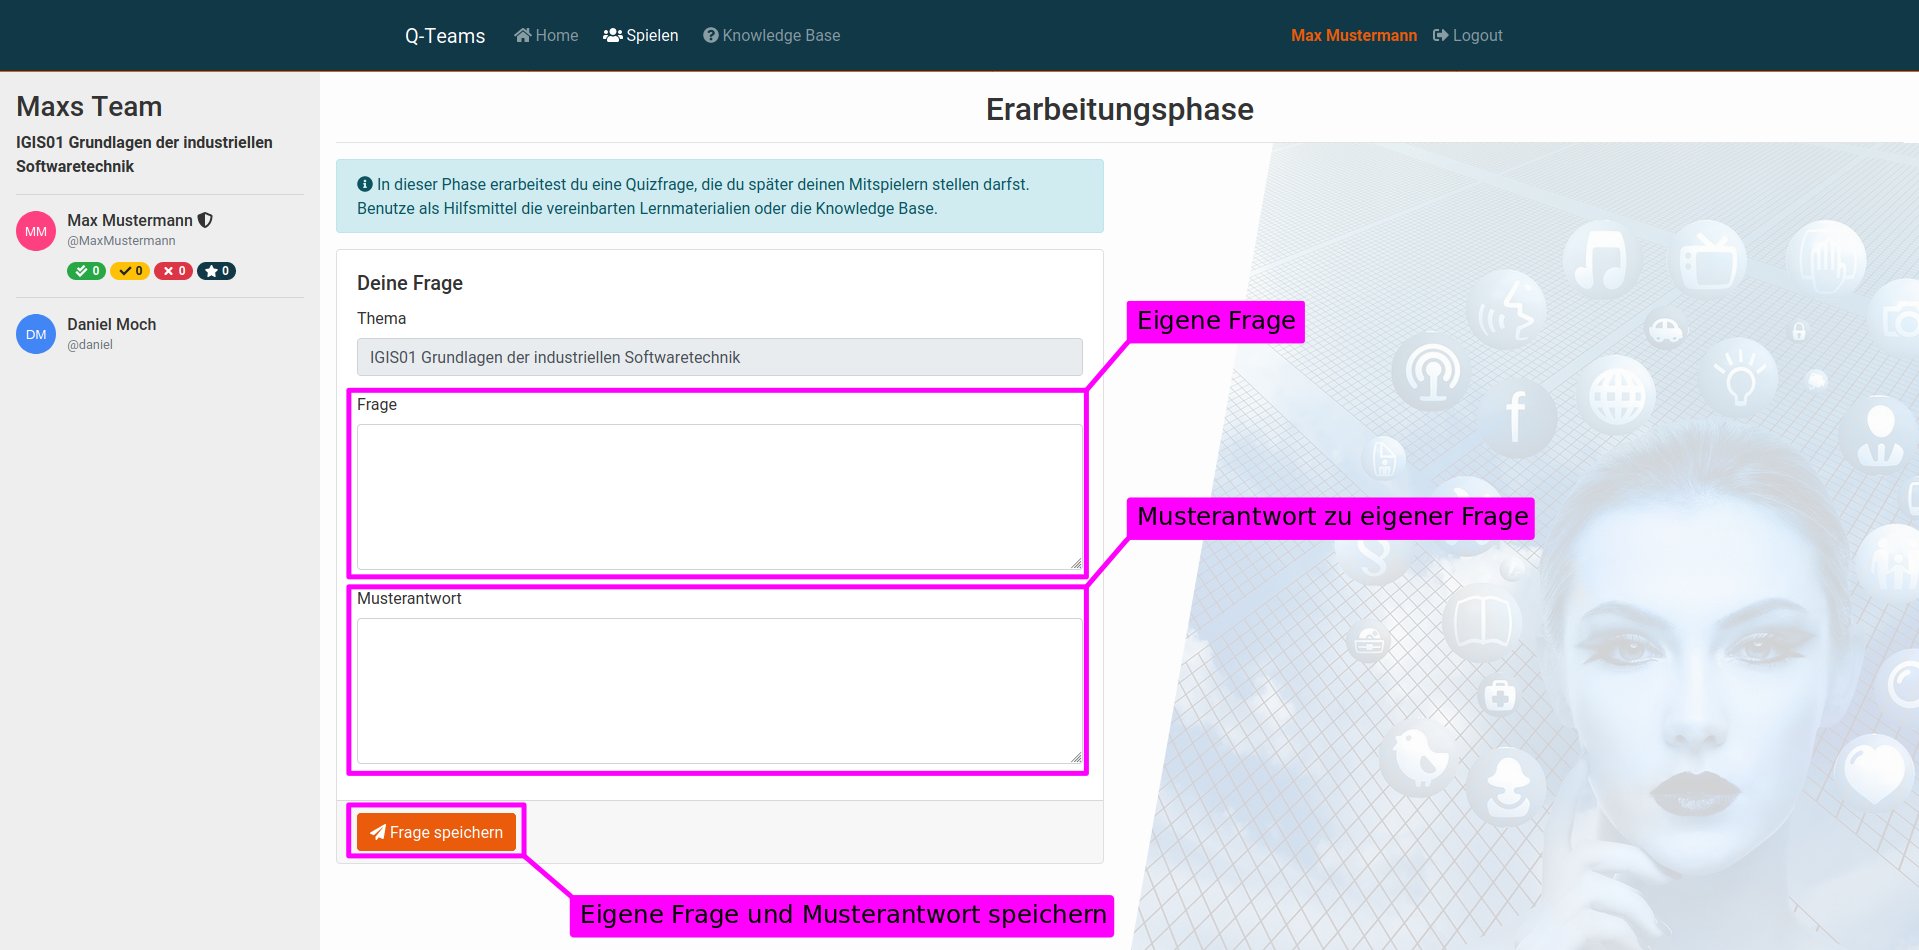
\includegraphics[width=\textwidth]{UserGuide/Erarbeitungsphase.png}
		\caption{Die Erarbeitungsphase}
		\label{fig:guide_erarbeitungsphase}
	\end{figure}	
	
	Alle anderen Spieler des Teams erstellen parallel zu dir die Frage und Antwort, solltest du schneller sein, gelangst du erstmal auf den Warten-Bildschirm aus Abbildung \ref{fig:guide_erarbeitungsphase_warten}. Haben alle Spieler ihre Frage gespeichert, beginnt die erste Fragephase.
	\begin{figure}[h!]
		\centering
		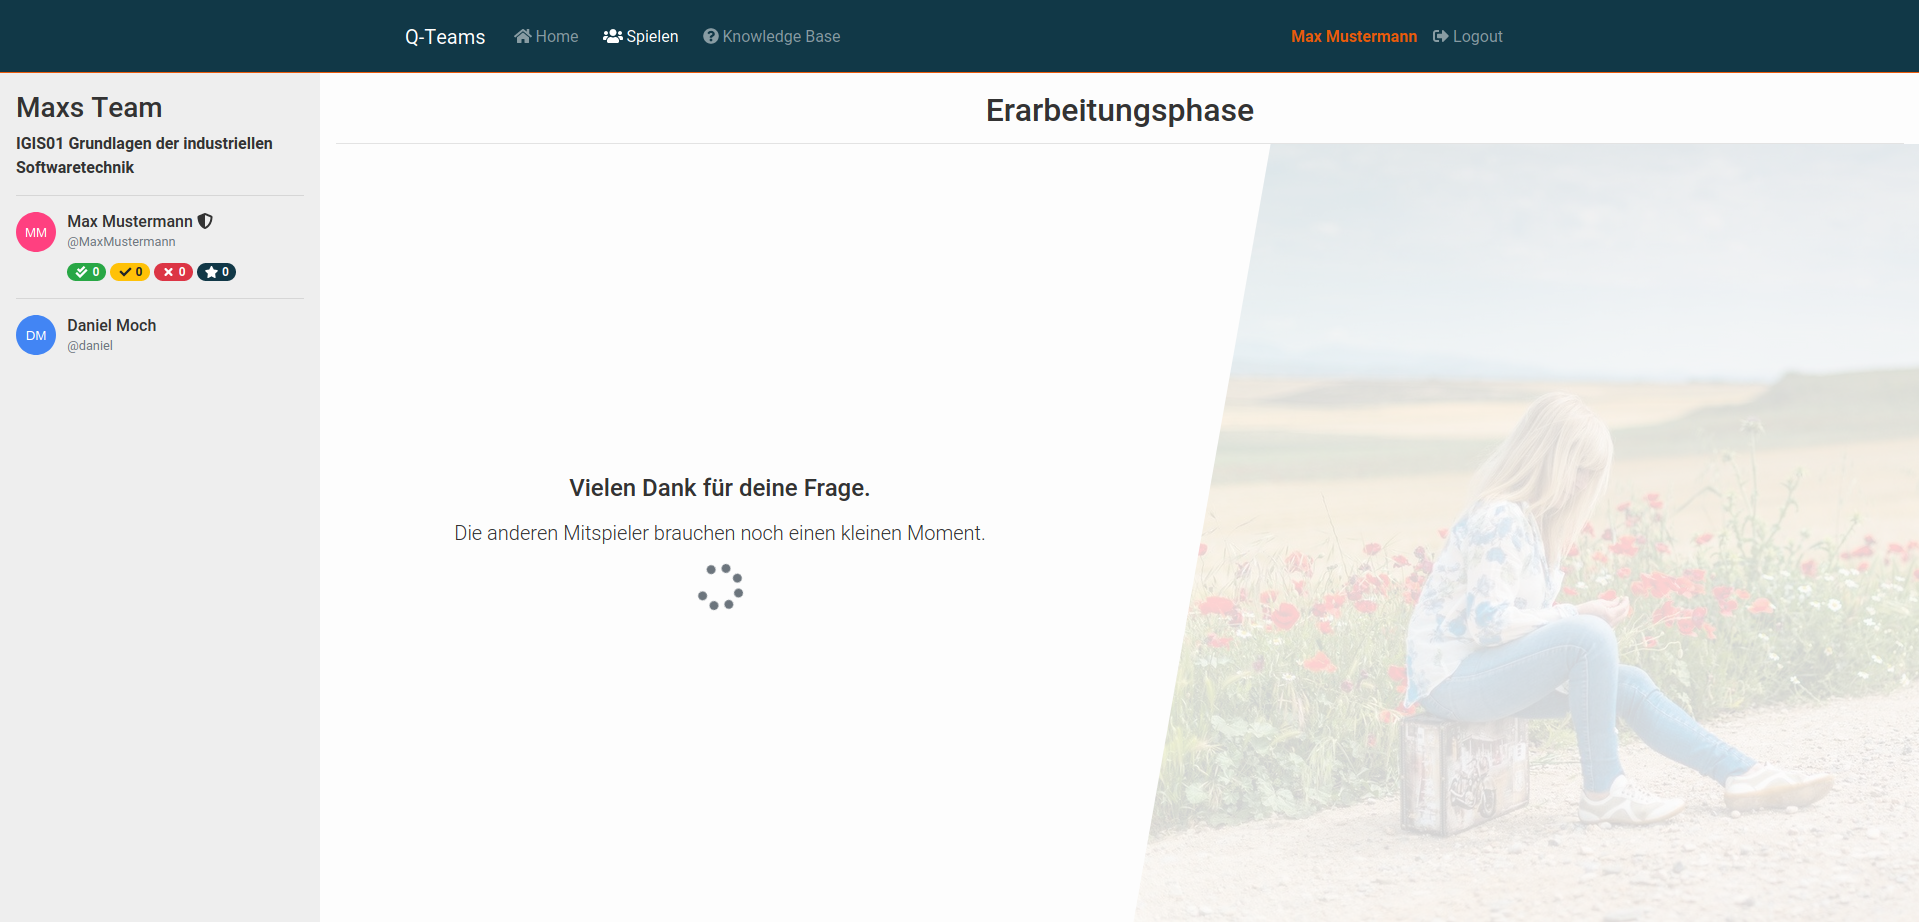
\includegraphics[width=\textwidth]{UserGuide/Erarbeitungsphase_warten.png}
		\caption{Die Erarbeitungsphase nach gespeicherter Frage}
		\label{fig:guide_erarbeitungsphase_warten}
	\end{figure}
	
	\newpage
	\section*{Schritt 6: Die Frage eines Mitspielers beantworten}
	
	Hast du die Frage eines Mitspielers zu beantworten, wird dir der Bildschirm aus Abbildung \ref{fig:guide_fragephase} angezeigt. Oben findest du die entsprechende Frage und den Namen des Fragestellers. Nun musst du deine Antwort zur Frage eingeben und anschließend deine Antwort durch Klicken auf den Button absenden. Sobald alle Mitspieler die Frage beantwortet und abgesendet haben, geht es zur Bewertungsphase.	
	\begin{figure}[h!]
		\centering
		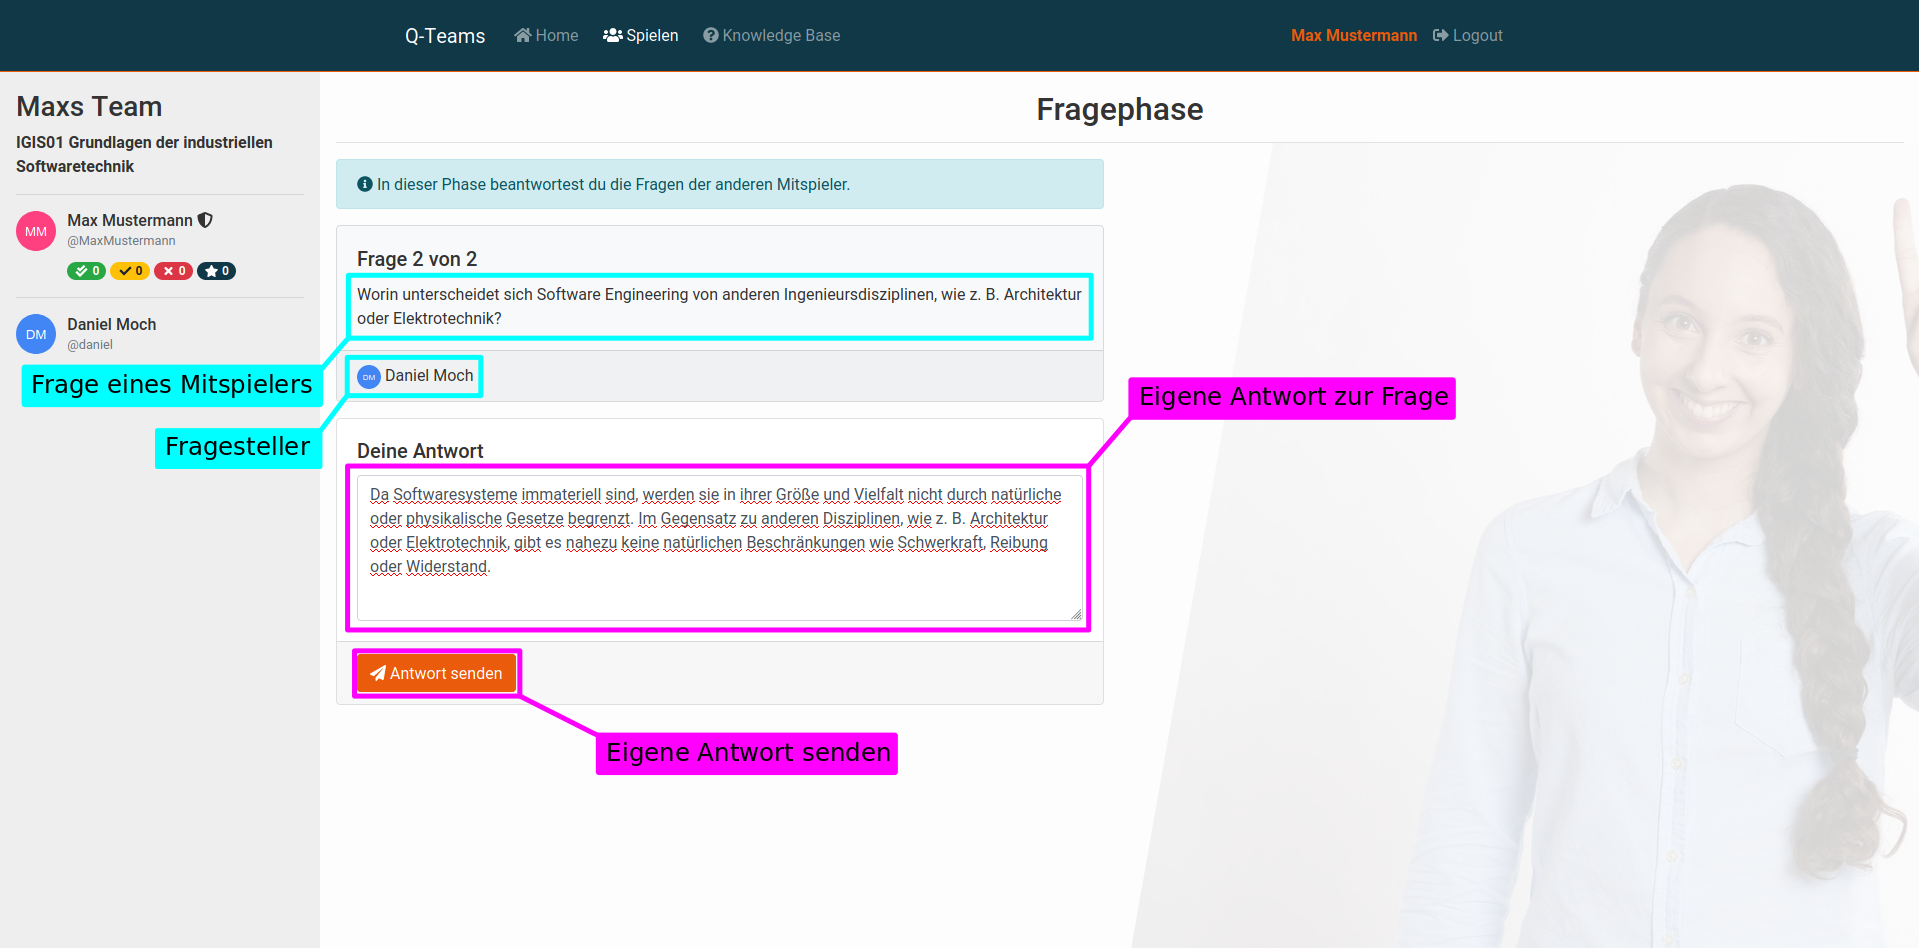
\includegraphics[width=\textwidth]{UserGuide/Fragephase_beantworten.png}
		\caption{Die Fragephase}
		\label{fig:guide_fragephase}
	\end{figure}
	
	Während die anderen Spieler deine Frage beantworten, kann der Fragesteller sich entspannen und auf die Bewertungsphase warten. Während der Wartezeit wird der Bildschirm im Abbildung \ref{fig:guide_fragephase_warten} angezeigt.
	
	\begin{figure}[h!]
		\centering
		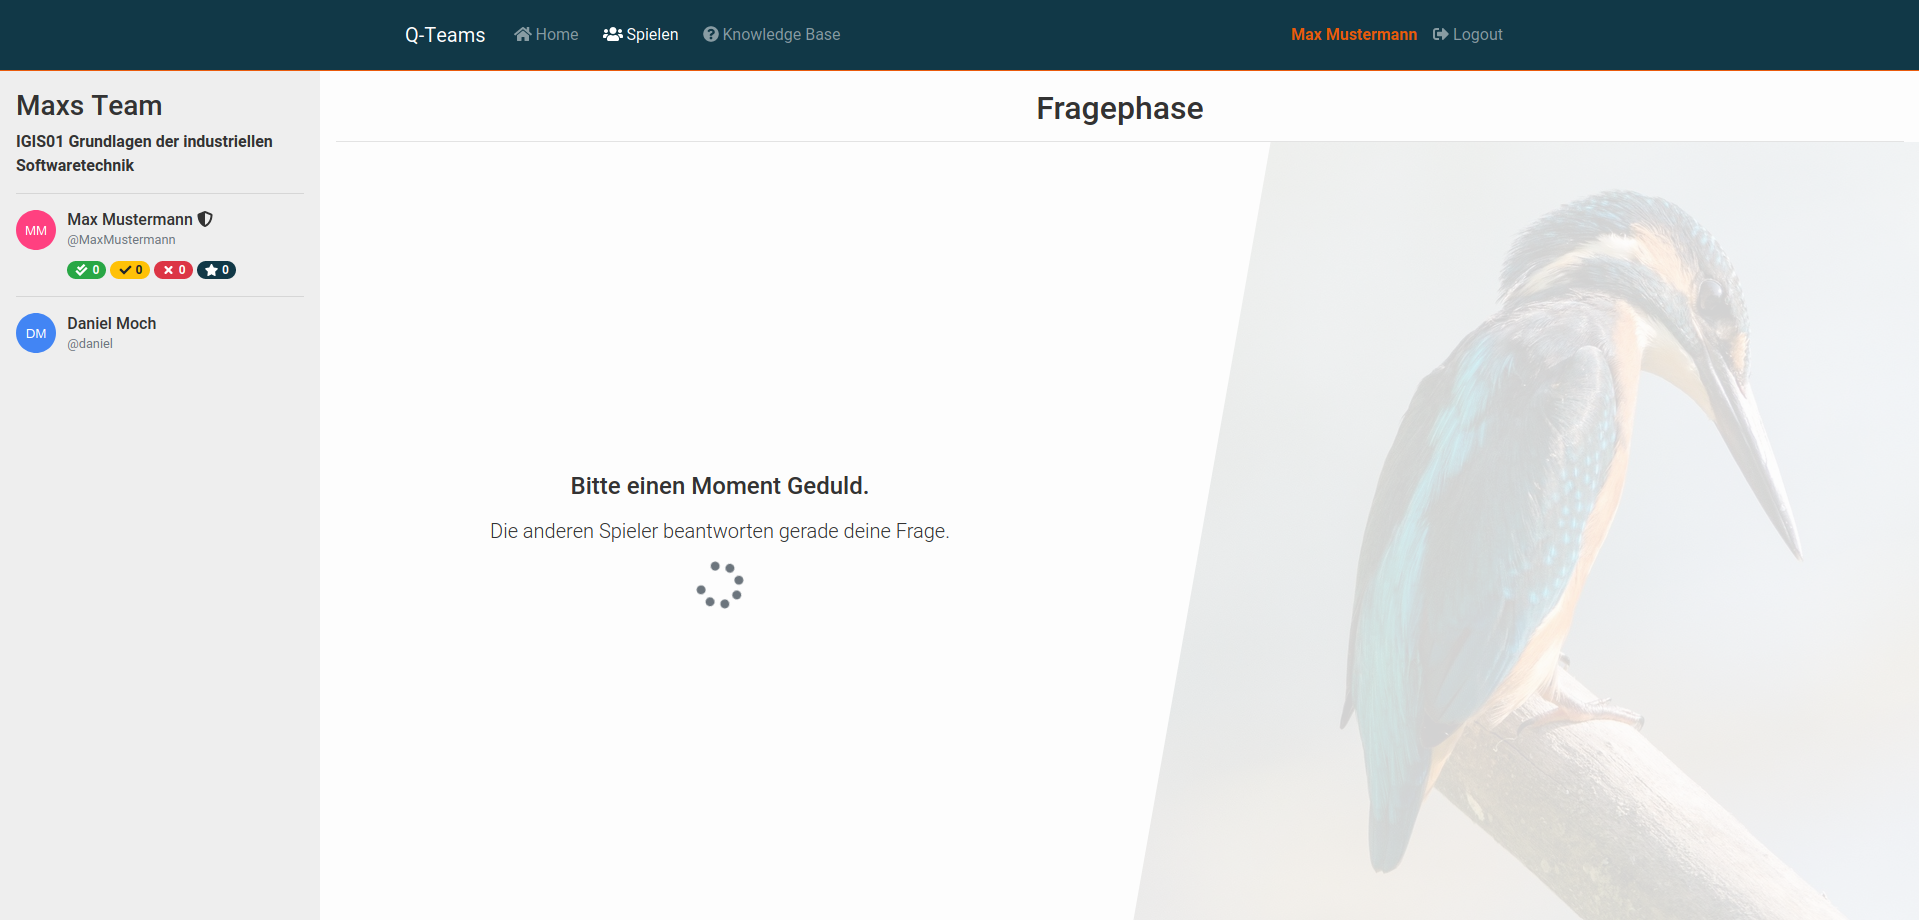
\includegraphics[width=\textwidth]{UserGuide/Fragephase_warten.png}
		\caption{Die Fragephase aus Sicht des Fragestellers}
		\label{fig:guide_fragephase_warten}
	\end{figure}
	
	\newpage
	\section*{Schritt 7: Die Antworten der Mitspieler bewerten}
					
	Sobald alle anderen Spieler deine Frage beantwortet haben musst du deren Antworten bewerten. Dazu wird dir der Bewertungsbildschirm angezeigt, siehe Abbildung \ref{fig:guide_bewertungsphase}.
	Ganz oben wird dir die Frage mit der passenden Musterantwort angezeigt. Darunter sind die Antworten deiner Mitspieler aufgelistet. Jede Antwort musst du nun mit richtig/teilweise richtig/falsch bewerten. Durch Klicken auf den Button \textit{Bewertungsphase abschließen} werden deine Bewertungen gespeichert und die nächste Fragephase wird gestartet. Wurden bereits alle Fragen beantwortet, ist diese Runde anschließend beendet und ihr startet wieder in der Phase \textit{Beginn des Spiels}.
	
	Die antwortenden Spieler sehen die Bewertungen des Fragestellers sofort und können, solange die Phase noch nicht abgeschlossen wurde, noch um eine bessere Bewertung feilschen.
	
	\begin{figure}[h!]
		\centering
		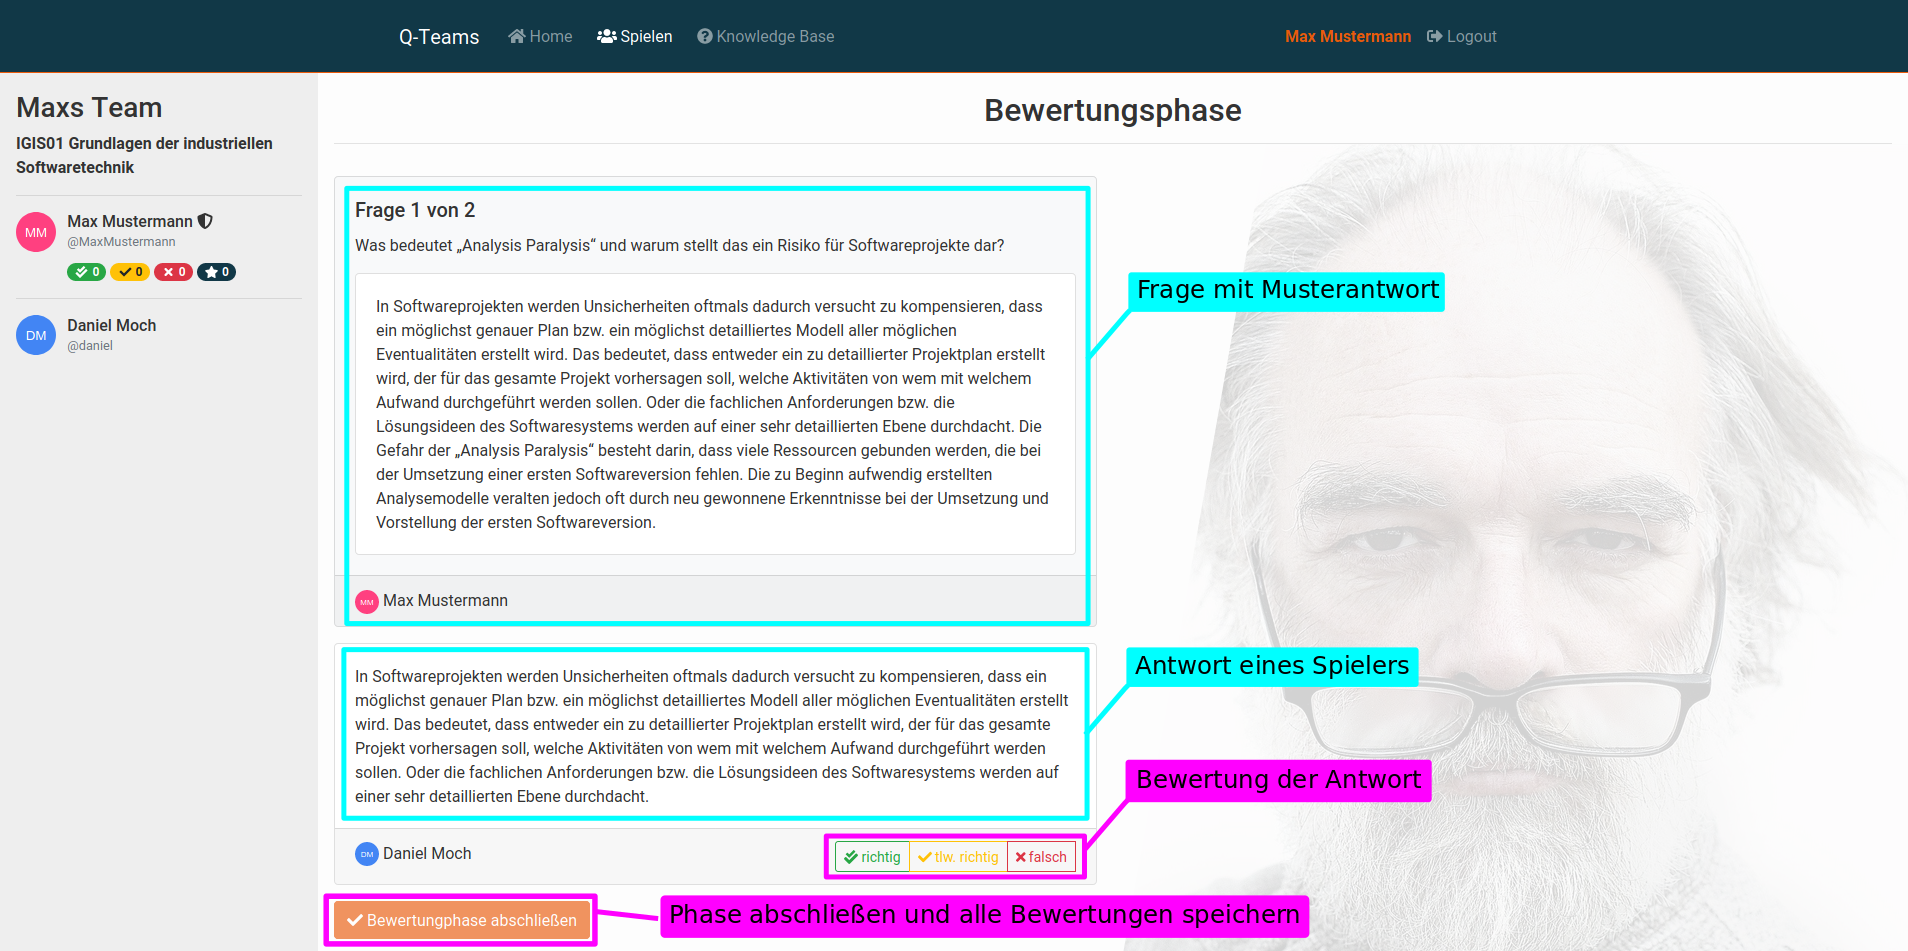
\includegraphics[width=\textwidth]{UserGuide/Bewertungsphase.png}
		\caption{Die Bewertungsphase}
		\label{fig:guide_bewertungsphase}
	\end{figure}
	
	\newpage
	\section*{Schritt 8: Die Knowledge Base nutzen}
						
	Um das volle Potenzial von Q-Teams zu nutzen, solltest du die Knowledge Base nutzen. Dazu klicke in der Top-Leiste auf den Button Knowledge Base. Dann wird dir der Startbildschirm der Knowledge Base angezeigt, siehe Abbildung \ref{fig:guide_kb_start}. In der Knowledge Base werden alle jemals gestellten Fragen und deren Musterantworten gespeichert. Um die Knowledge Base zu durchsuchen, kannst du entweder einen oder mehrere Suchbegriffe eingeben, aus der Gesamtliste der Themen auswählen oder dir die Themen mit den meisten gespeicherten Fragen anschauen.				
						
	\begin{figure}[h!]
		\centering
		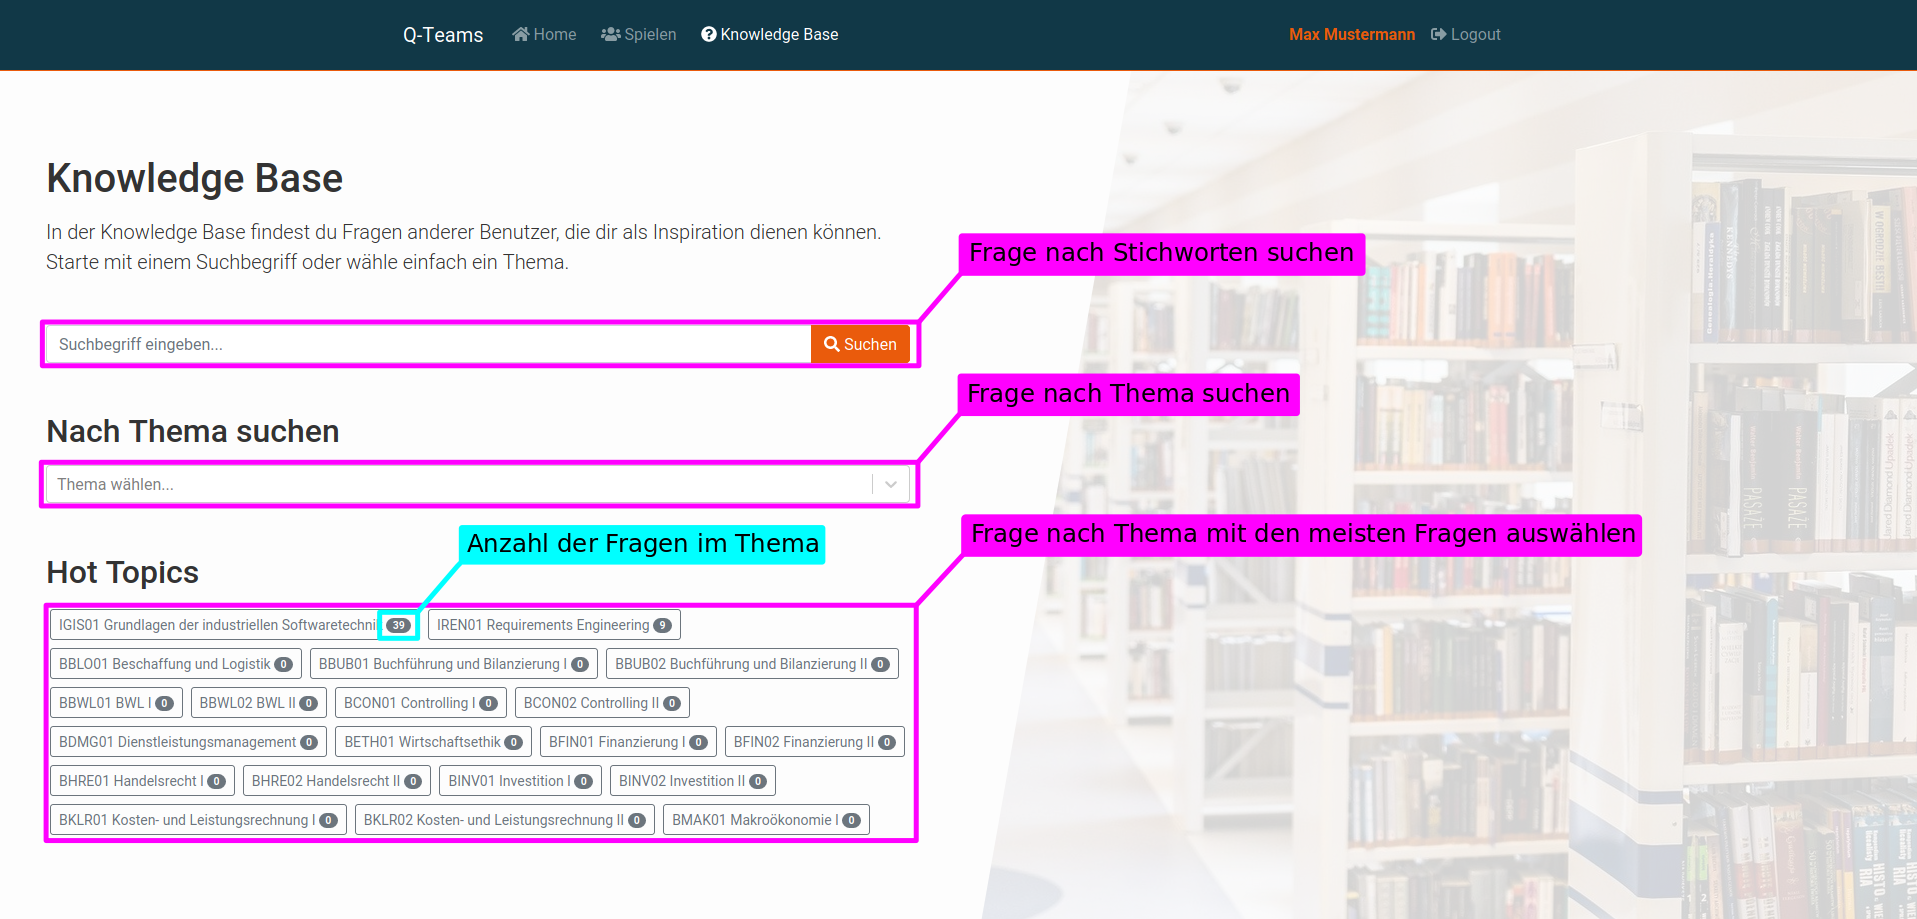
\includegraphics[width=\textwidth]{UserGuide/Knowledge_Base_start.png}
		\caption{Der Startbildschirm der Knowledge Base}
		\label{fig:guide_kb_start}
	\end{figure}	
	
	Die Fragen werden dir dann wie in Abbildung \ref{fig:guide_kb} angezeigt. Alle Fragen, die deinen Suchkriterien entsprechen, werden aufgelistet. Zu jeder Frage wird auch der Ersteller angezeigt, an ihn kannst du durch Klicken auf den Briefumschlag-Button eine Nachricht schicken. Solltest du einen Fehler in der Frage gefunden haben oder Verbesserungsvorschläge haben, benachrichtige den Ersteller!
	
	\begin{figure}[h!]
		\centering
		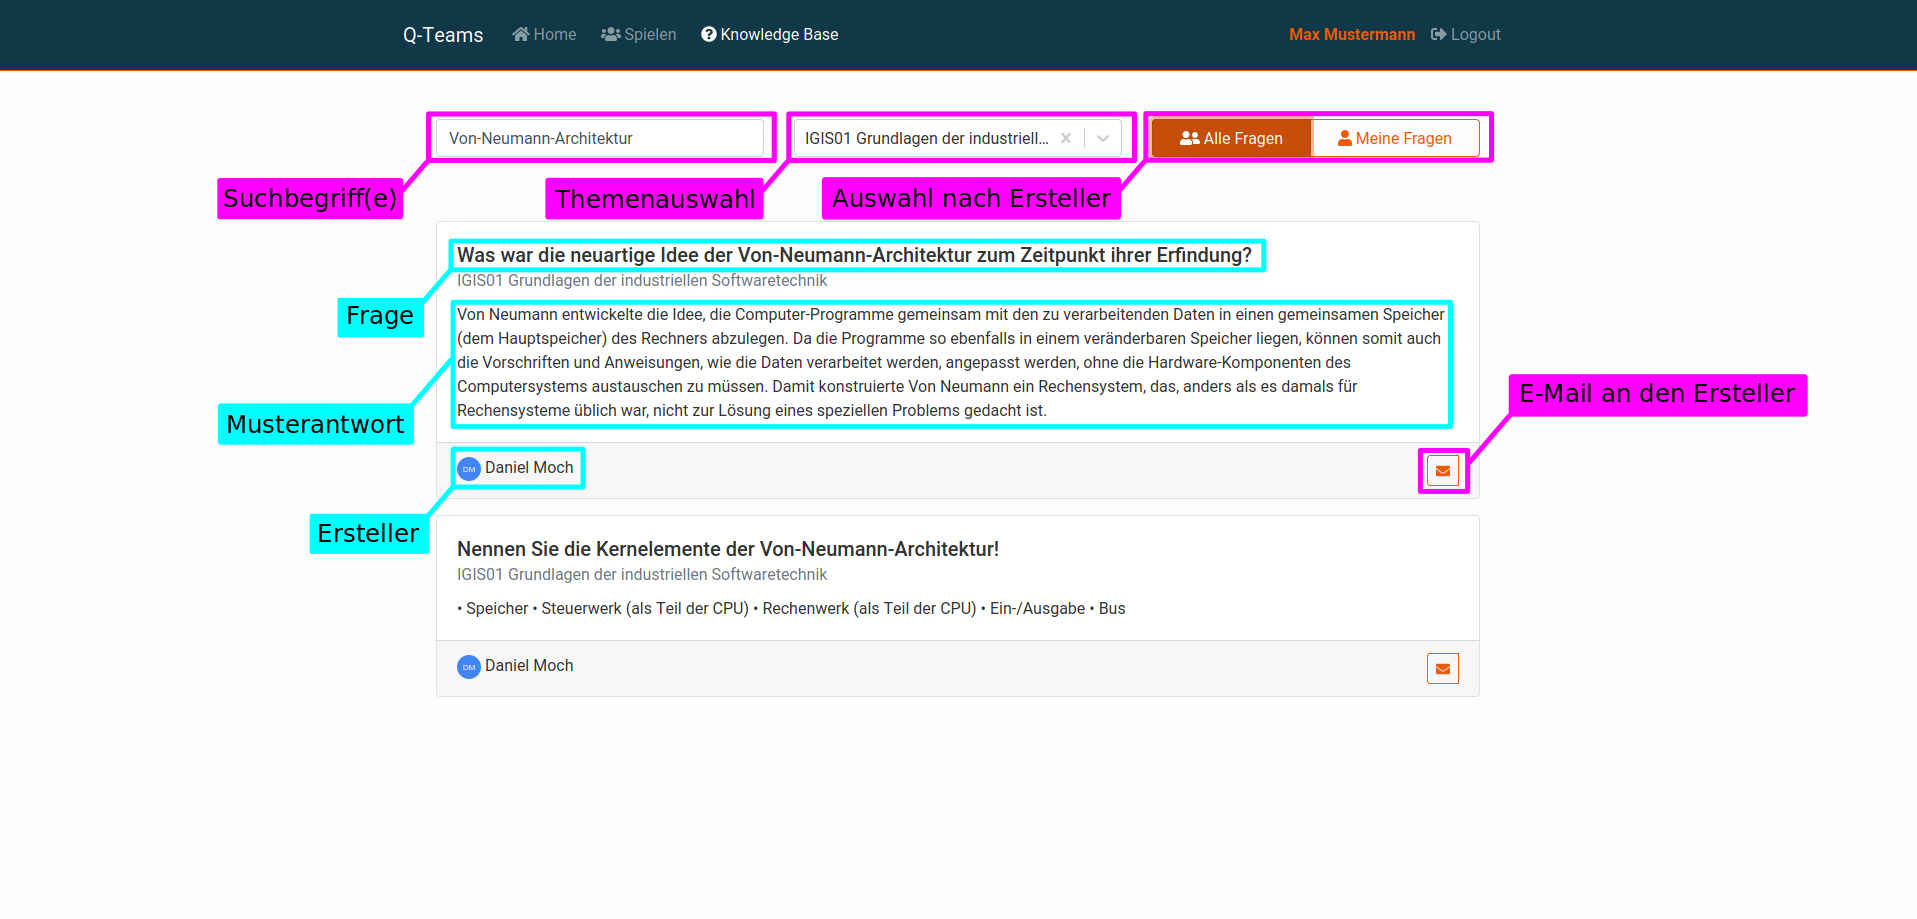
\includegraphics[width=\textwidth]{UserGuide/Knowledge_Base.png}
		\caption{Die Knowledge Base}
		\label{fig:guide_kb}
	\end{figure}	
	
	Auch auf diesem Bildschirm kannst du deine Suchkriterien angeben, \dash Suchbegriff(e) oder Thema. Außerdem hast du die Möglichkeit nach eigenen Fragen zu filtern, dazu klicke auf den Button \textit{Meine Fragen}. Deine eigene Fragen kannst du ändern oder auch löschen, siehe Abbildung \ref{fig:guide_kb_eigene}.
		
	\begin{figure}[h!]
		\centering
		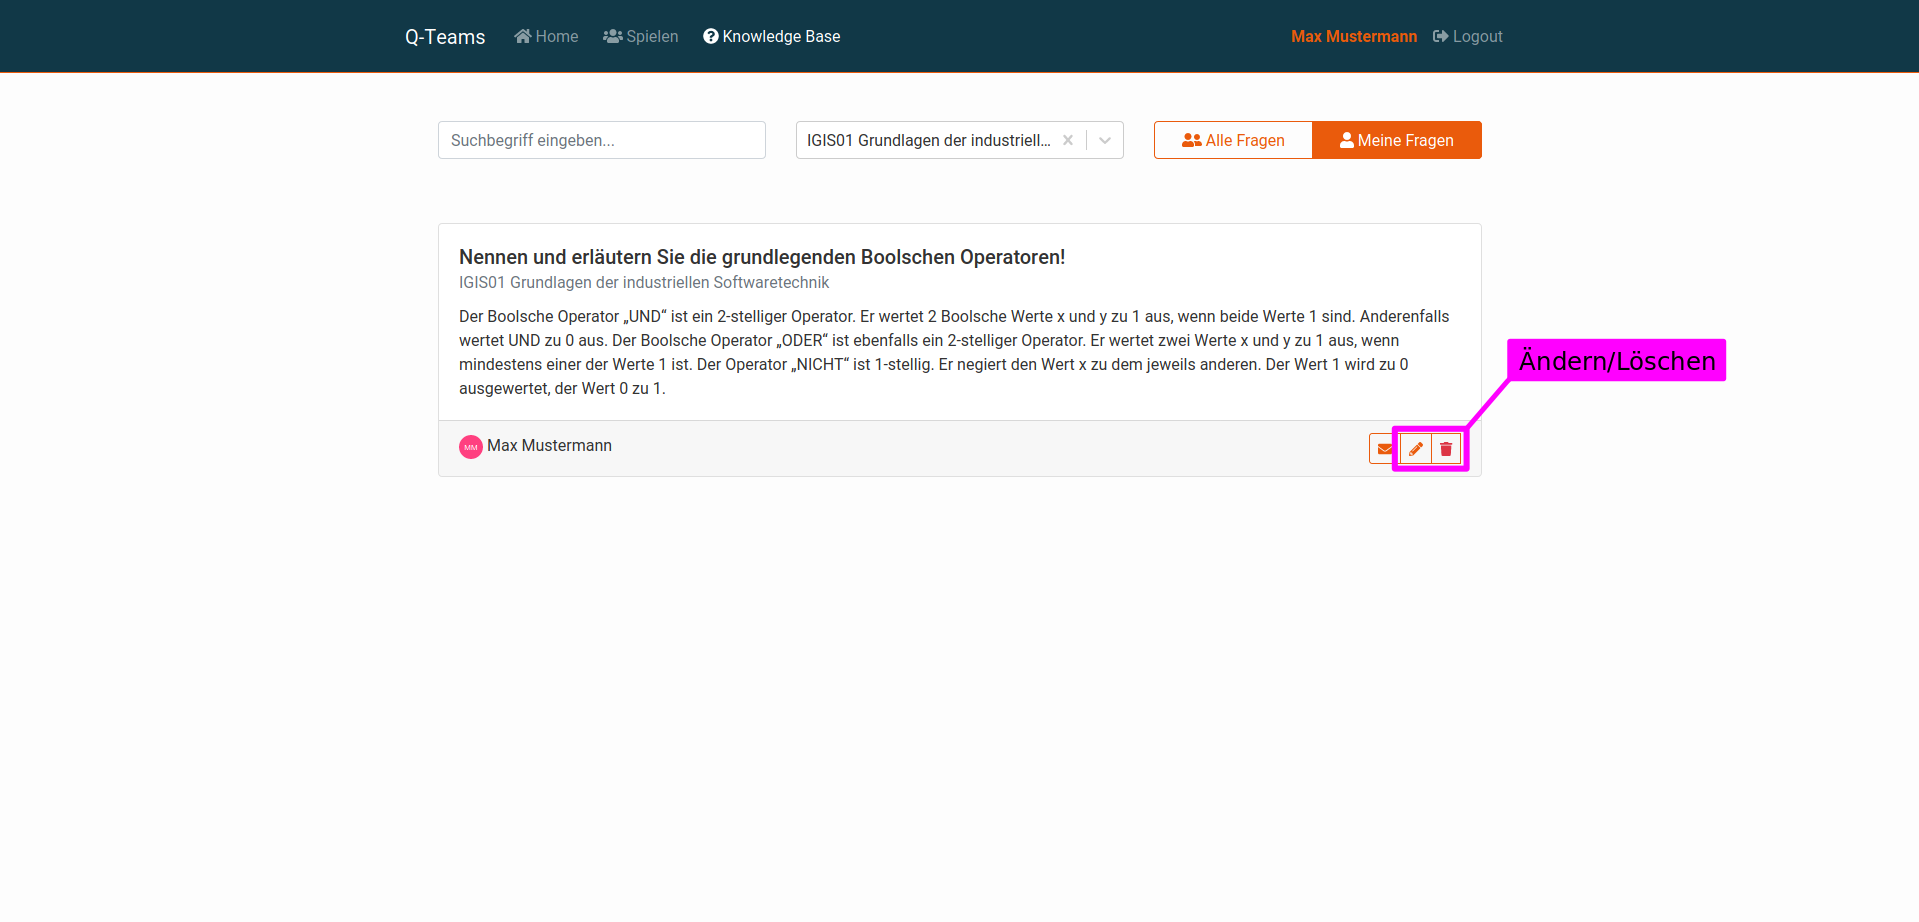
\includegraphics[width=\textwidth]{UserGuide/Knowledge_Base_eigene.png}
		\caption{Die Knowledge Base mit eigenen Fragen}
		\label{fig:guide_kb_eigene}
	\end{figure}	
			
	

	\chapter{Administration}
	Das Q-Teams-Projekt ist so konzipiert, dass nahezu keine administrativen Tätigkeiten erforderlich sind.
	
	Insbesondere die Benutzerverwaltung muss jedoch derzeit noch von einem Administrator durchgeführt werden. Dies entfällt, sobald das System an das Single-Sign-On-System der IUBH angebunden ist.
	
	Die Liste der Themen (Modulbezeichnungen und -nummern) wurde über eine Textdatei aus dem Interactive Book Reader der IUBH importiert. Sie kann manuell vom Administrator ergänzt werden.

	Sollen Fragen anderer Nutzer aus der Knowledge Base geändert oder gelöscht werden, so ist dies ebenfalls über die Administrationsoberfläche möglich. 	
		
	\section{Anmeldung und Übersichtsseite}
	Die Administrationsoberfläche von Q-Teams ist unter der Adresse  \url{https://api.qteams.team/admin}	erreichbar. Nach dem Login mit einem Administratorkonto präsentiert sich die in Abbildung \ref{fig:admin} dargestellte Übersichtsseite der Django-Verwaltung.
	
	\begin{figure}[h!]
		\centering
		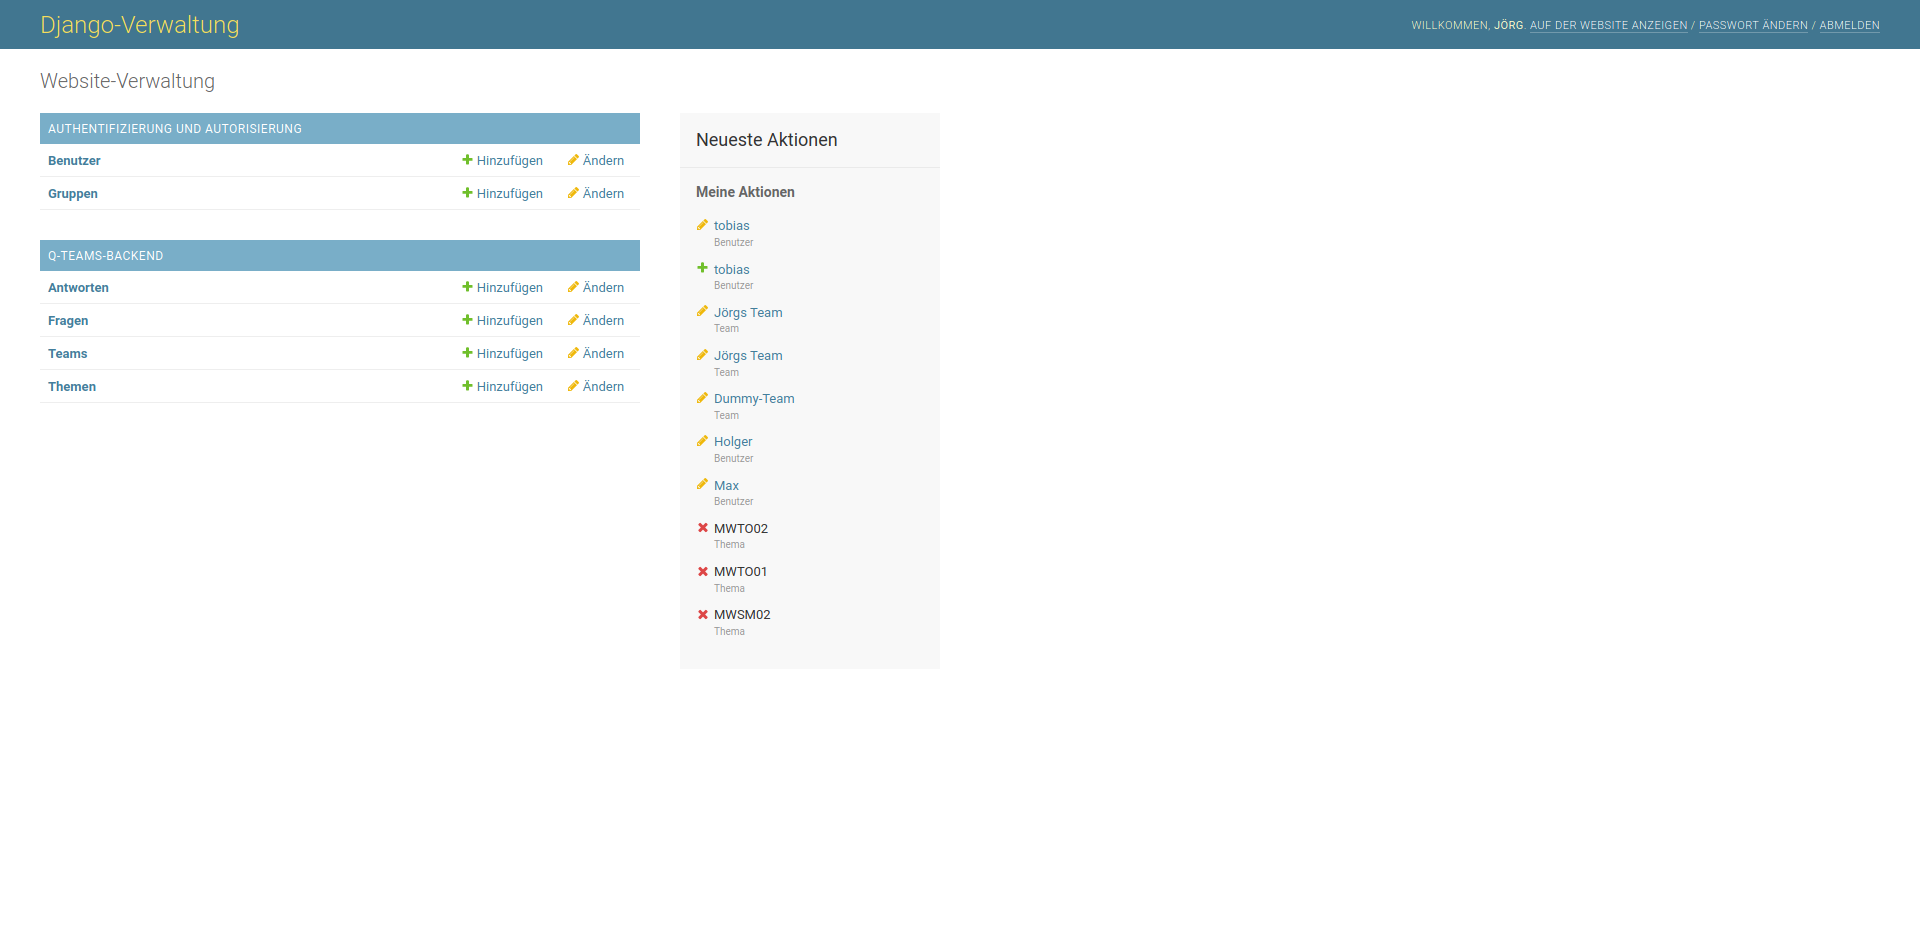
\includegraphics[width=\textwidth]{admin}
		\caption{Administrationsoberfläche}
		\label{fig:admin}
	\end{figure}
	
	Im Bereich \textit{Authentifizierung und Autorisierung} können Benutzer und Benutzergruppen verwaltet werden. Die Benutzergruppen werden derzeit im Projekt nicht verwendet.
	
	Im Bereich \textit{Q-Teams-Backend} finden sich die fachlichen Entitäten des Quizsystems. In der Regel ist hier keine manuelle Intervention erforderlich. Im Folgenden werden daher nur die Bereiche \textit{Fragen} und \textit{Themen} kurz beschrieben. 
	
	\section{Benutzerverwaltung}
	
	\begin{figure}
		\centering
		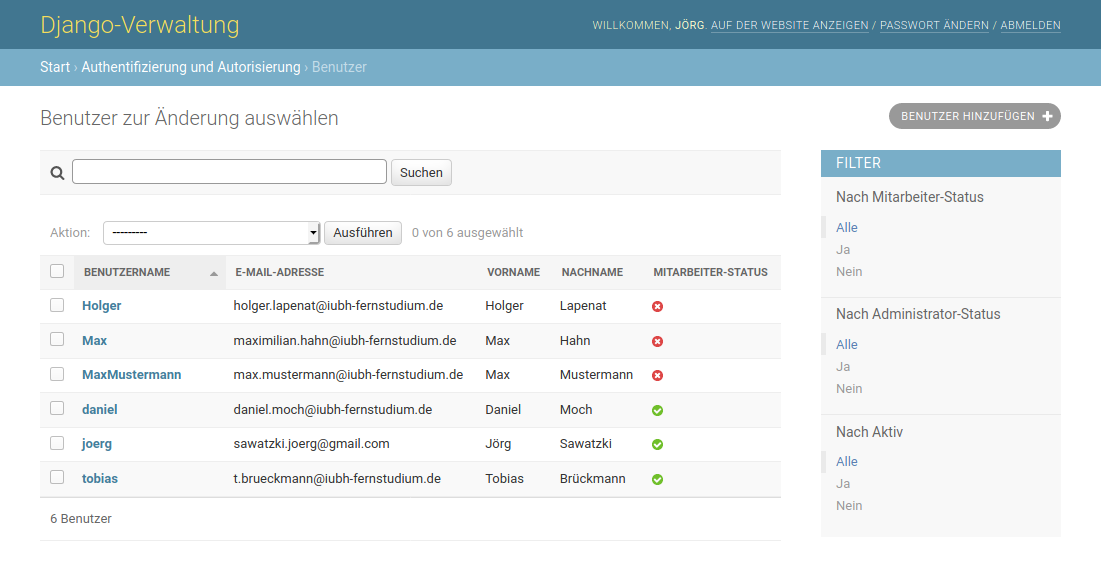
\includegraphics[width=\textwidth]{benutzer}
		\caption{Übersichtsseite der Benutzerverwaltung}
		\label{fig:benutzer}
	\end{figure}
	
	Die Benutzerverwaltung ist erreichbar über den Link \textit{Benutzer} im Abschnitt \textit{Authentifizierung und Autorisierung} der Übersichtsseite.
	
	Abbildung \ref{fig:benutzer} zeigt die Übersichtsseite der Benutzerverwaltung.
	
	Über den Button \textit{Benutzer hinzufügen} kann ein neuer Benutzer erstellt werden. Zunächst muss dabei ein Benutzername und ein sicheres Passwort vergeben werden, das verschlüsselt in der Datenbank abgespeichert wird -- vgl. dazu Abbildung \ref{fig:neuerbenutzer}.
	
	\begin{figure}
		\centering
		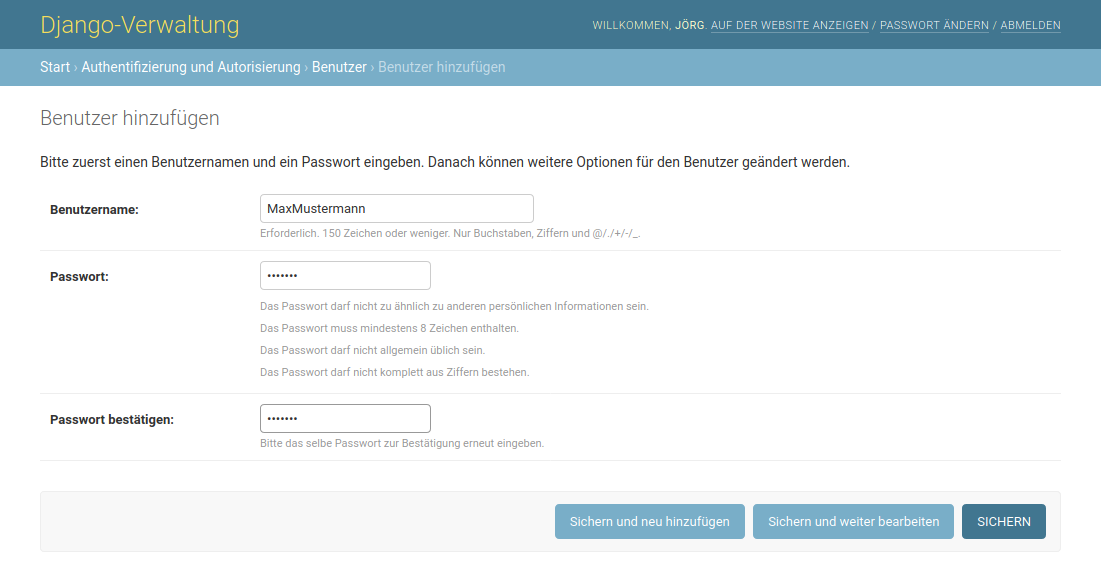
\includegraphics[width=\textwidth]{neuerbenutzer}
		\caption{Anlegen eines Benutzers}
		\label{fig:neuerbenutzer}
	\end{figure}
	
	\begin{figure}
		\centering
		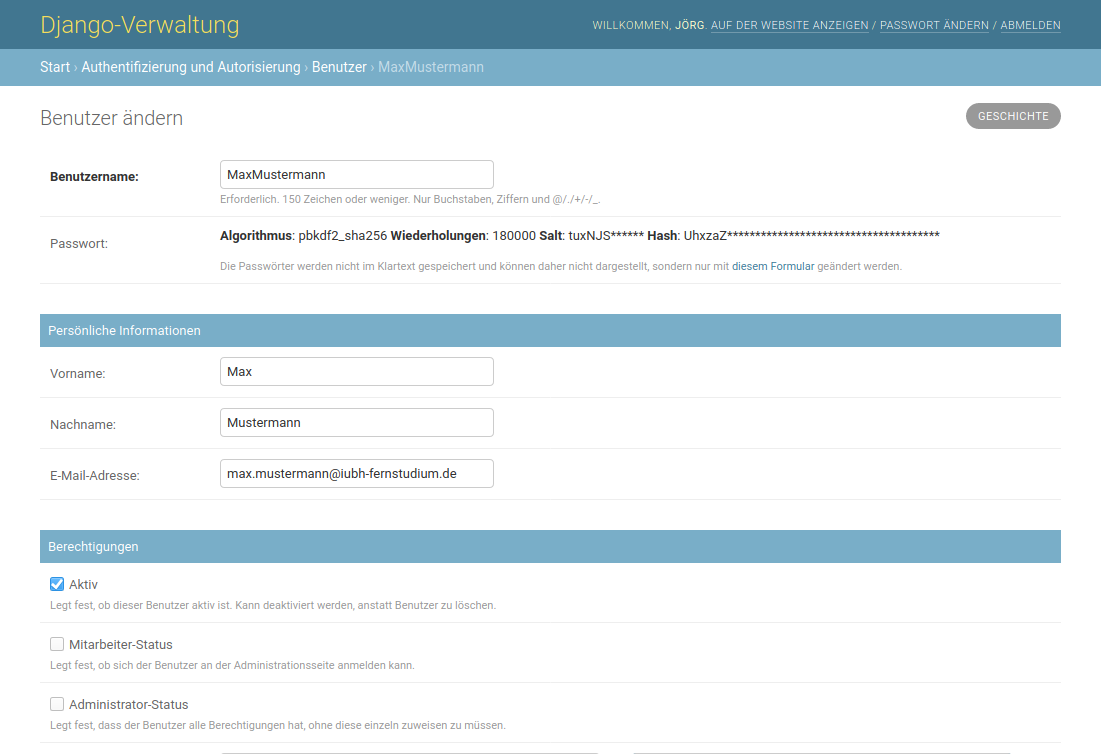
\includegraphics[width=\textwidth]{editbenutzer}
		\caption{Benutzerkonto bearbeiten}
		\label{fig:editbenutzer}
	\end{figure}
	
	Sind Passwort und Benutzername vergeben, so öffnet sich die Seite \textit{Benutzer bearbeiten}, die später auch über einen Klick auf den Benutzernamen in der Tabelle der Übersichtsseite aufgerufen werden kann.
	
	Über die Seite \textit{Benutzer bearbeiten} (siehe Abbildung \ref{fig:editbenutzer}) müssen mindestens Vorname und Nachname gesetzt werden, damit der Benutzer im Quiz korrekt angezeigt werden kann.
	
	Soll der Benutzer administrative Tätigkeiten ausführen können, so muss bei \textit{Mitarbeiter-Status} und \textit{Administrator-Status} ein Häkchen gesetzt werden -- andernfalls kann er lediglich das Quiz spielen, sich jedoch nicht in der Verwaltung anmelden.
	
	Das Entfernen eines Benutzerkontos kann über den Button \textit{Löschen} auf der Seite \textit{Benutzer bearbeiten} oder alternativ auf der Übersichtsseite erfolgen.
	
	\section{Themenverwaltung}
	Über den Link \textit{Themen} im Bereich \textit{Q-Teams-Backend} können neue Module hinzugefügt oder vorhandene aktualisiert bzw. gelöscht werden. Die Bedienung funktioniert analog zur Benutzerverwaltung.
	
	Abbildung \ref{fig:editthema} zeigt beispielhaft das Editieren eines Themas.
	
	\begin{figure}
		\centering
		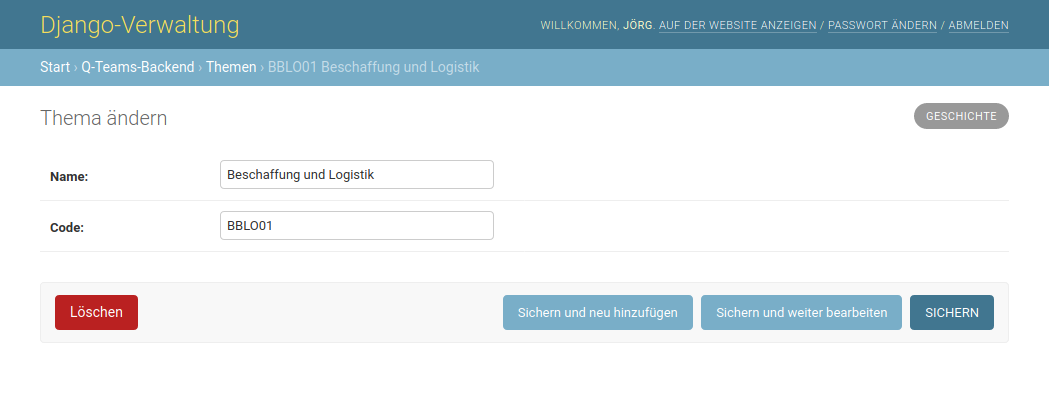
\includegraphics[width=\textwidth]{editthema}
		\caption{Ändern eines Themas}
		\label{fig:editthema}
	\end{figure}
	
	\section{Fragenverwaltung}
	In der Regel verwalten die Benutzer ihre Fragen selbstständig und es ist kein Eingreifen erforderlich. Sollte dennoch einmal der Fragenkatalog aufgeräumt werden müssen, so ist dies über den Link \textit{Fragen} im Bereich \textit{Q-Teams-Backend} problemlos möglich. 
	
	Abbildung \ref{fig:editfrage} zeigt beispielhaft das Editieren einer Frage.
	
	\begin{figure}
		\centering
		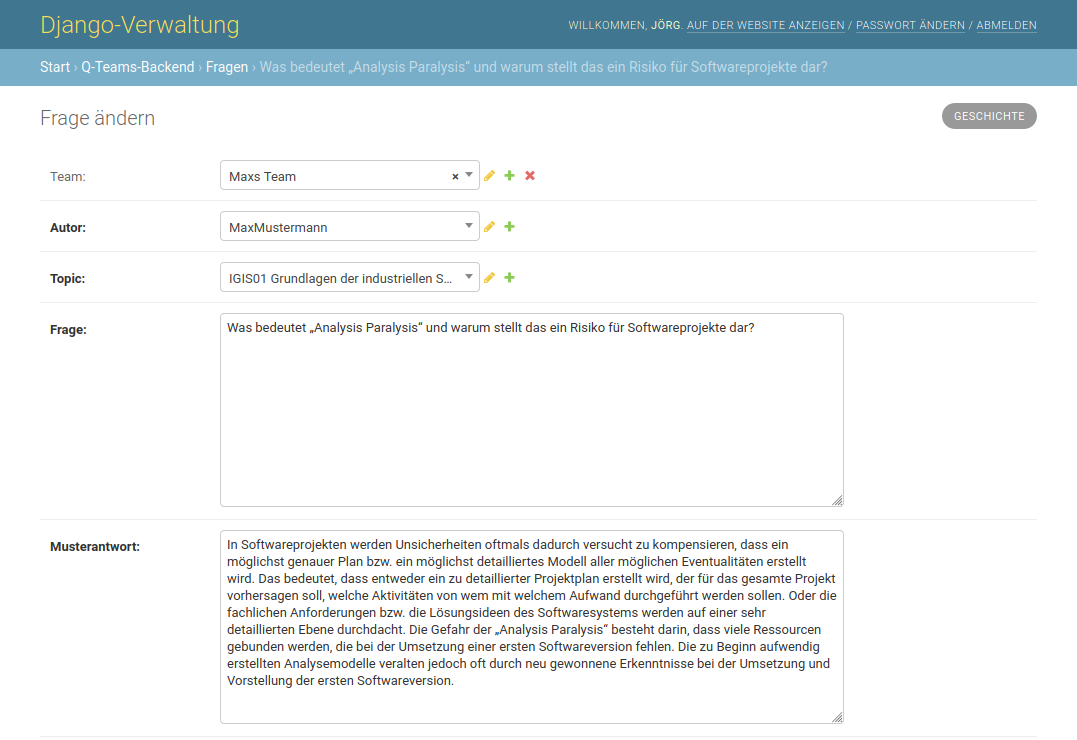
\includegraphics[width=\textwidth]{editfrage}
		\caption{Ändern einer Frage}
		\label{fig:editfrage}
	\end{figure}
	
	\chapter{Installation und Inbetriebnahme}
	Für die Installation wird ein linuxbasiertes Serversystem benötigt. Die Installation und Inbetriebnahme des Frontends und des Backends werden in den folgenden Abschnitten separat beschrieben.
	
	\section{Frontend}
	
	Das Frontend besteht aus statischen HTML-, CSS- und JS-Dateien, die von einem beliebigen Webserver bereitgestellt werden können.
	Es wird vorausgesetzt, dass der grundlegende Umgang mit dem Versionskontrollsystem Git bekannt ist.
	
	Mit folgendem Befehl kann der Quellcode ausgecheckt und in das Quellcode-Verzeichnis gewechselt werden:		
	\begin{minted}{bash}
git clone https://github.com/joerg86/quiz_frontend.git
cd quiz_frontend
	\end{minted}
	
	Nun muss lediglich das Unterverzeichnis \texttt{build} auf einen Webserver kopiert werden. Wichtig dabei ist, dass der Webserver alle URLs außerhalb des Pfades \texttt{/static} auf die Datei \texttt{index.html} umleitet, da das URL-Routing clientseitig abläuft.
	
	Dies kann bei Apache beispielsweise mit dem Modul \textit{mod\_{}rewrite} und einer \textit{.htacces}-Datei geschehen, die in Listing \ref{lst:rewrite} beispielhaft dargestellt ist:
	\begin{listing}
	\begin{minted}{apacheconf}
RewriteEngine On
RewriteBase /
RewriteCond "\%{HTTP_HOST}" "^qteams.team\$" 
RewriteRule "^static/(.*)\$" "qteams.team/static/\$1" [END]
RewriteCond "\%{HTTP_HOST}" "^qteams.team\$" 
RewriteRule "^(.*)\$" "qteams.team/index.html" [END]
	\end{minted}
		\caption{.htaccess-Datei für das Frontend}
		\label{lst:rewrite}
	\end{listing}
	
	Sollen weitere Anpassungen vorgenommen werden, z.B. die API-URL des Backend-Servers geändert werden (Standardeinstellung ist \texttt{api.qteams.team}), so muss zunächst die Datei \texttt{dotenv.production} angepasst und die URLs entsprechend verändert werden.
	
	Um die Änderungen zu übernehmen, muss das Projekt neu kompiliert werden. Dazu muss eine NodeJS-Umgebung\footnote{https://nodejs.org} und der Paketmanager Yarn\footnote{https://yarnpkg.com/} installiert werden.
	
	Danach kann das Projekt mit den Befehlen \mintinline{bash}{yarn install} und \mintinline{bash}{yarn build} neu übersetzt und der \texttt{build}-Ordner auf den Webserver kopiert werden.
	
	\section{Backend}
	Für die Installation und Inbetriebnahme des Backends wird ein Python-Interpreter in der Version 3.7 oder höher benötigt und Grundkenntnisse im Umgang mit virtuellen Python-Umgebungen und dem Paketmanager \textit{pip} vorausgesetzt.
	
	Mit folgendem Befehl kann der Quellcode ausgecheckt und in das Quellcode-Verzeichnis gewechselt werden:		
	\begin{minted}{bash}
git clone https://github.com/joerg86/quiz_backend.git
cd quiz_backend
	\end{minted}
	
	Nun muss eine virtuelle Python-Umgebung erstellt und die für das Projekt benötigten Python-Bibliotheken installiert werden:
	\begin{minted}{bash}
virtualenv env -p python3
source env/bin/activate
pip install -r requirements.txt
	\end{minted}
	
	Das Projekt verwendet standardmäßig das Datenbanksystem \textit{SQLite}. Soll ein anderes Datenbanksystem (z.\,B. MySQL oder PostgreSQL) verwendet werden, so muss an dieser Stelle ein entsprechender Datenbankserver eingerichtet werden und der Zugang in der Datei \texttt{qteams/settings.py} konfiguriert werden -- näheres dazu findet sich in der Django-Dokumentation\footnote{https://docs.djangoproject.com/en/3.0/ref/databases/}. Für die Einrichtung von SQLite sind keine weiteren Schritte erforderlich.
	
	Mit folgenden Befehlen wird die Datenbank vorbereitet und die statischen Assets bereitgestellt:
	
	\begin{minted}{bash}
python manage.py migrate
python manage.py collectstatic
	\end{minted}
	
	Nun kann ein Administratorkonto erstellt werden:
	
	\begin{minted}{bash}
python manage.py createsuperuser
	\end{minted}
	
	An dieser Stelle ist die Applikation fertig eingerichtet. Sie kann nun über den Daphne-Application-Server\footnote{https://github.com/django/daphne} zur Verfügung gestellt werden. 
	
	Daphne wurde bereits zusammen mit den anderen Python-Abhängigkeiten installiert und kann gestartet werden mit:
	
	\begin{minted}{bash}
daphne qteams.asgi:application
	\end{minted}
	
	Die Backend-API ist dann über \texttt{http://localhost:8000} erreichbar, die Administrationsoberfäche über \texttt{http://localhost:8000/admin/}.
	
	Es empfiehlt sich, den Dienst über ein Prozesskontrollsystem wie \textit{Supervisor}\footnote{http://supervisord.org/} zu verwalten. Listing \ref{lst:supervisor} zeigt eine beispielhafte Konfiguration dafür.
	
	\begin{listing}
		\begin{minted}{ini}
[program:quiz]
command=/home/joergs/quiz_backend/env/bin/daphne -s api.qteams.team qteams.asgi:application
autostart=true
autorestart=true
stderr_logfile = ~/quiz_backend/logs/err.log
stdout_logfile = ~/quiz_backend/logs/out.log
stopsignal=INT
environment=PYTHONPATH=/home/joergs/quiz_backend/
		\end{minted}
		\caption{Beispielhafte Supervisor-Konfigurationsdatei}
		\label{lst:supervisor}
	\end{listing}
	
	Weiterhin empfiehlt es sich, vor den Daphne-Server zur Absicherung einen Webserver wie NGINX oder Apache als Reverse Proxy zu schalten. Dazu sei auf die Dokumentation des entsprechenden Webservers verwiesen.
	

	
	\end{appendices}
	\newpage	
	\setcounter{chapter}{\thelastRomanCounter} % Fortsetzen der römischen Kapitelnummerierung
\renewcommand \thechapter{\Roman{chapter}}	\printbibliography[heading=bibnumbered,title=Literaturverzeichnis]

\end{document}
